%%%%%%%%%%%%%%%%%%%%%%% file template.tex %%%%%%%%%%%%%%%%%%%%%%%%%
%
% This is a general template file for the LaTeX package SVJour3
% for Springer journals.          Springer Heidelberg 2010/09/16
%
% Copy it to a new file with a new name and use it as the basis
% for your article. Delete % signs as needed.
%
% This template includes a few options for different layouts and
% content for various journals. Please consult a previous issue of
% your journal as needed.
%
%%%%%%%%%%%%%%%%%%%%%%%%%%%%%%%%%%%%%%%%%%%%%%%%%%%%%%%%%%%%%%%%%%%
%
% First comes an example EPS file -- just ignore it and
% proceed on the \documentclass line
% your LaTeX will extract the file if required
\begin{filecontents*}{example.eps}
%!PS-Adobe-3.0 EPSF-3.0
%%BoundingBox: 19 19 221 221
%%CreationDate: Mon Sep 29 1997
%%Creator: programmed by hand (JK)
%%EndComments
gsave
newpath
  20 20 moveto
  20 220 lineto
  220 220 lineto
  220 20 lineto
closepath
2 setlinewidth
gsave
  .4 setgray fill
grestore
stroke
grestore
\end{filecontents*}
%
\RequirePackage{fix-cm}
%
%\documentclass{svjour3}                     % onecolumn (standard format)
%\documentclass[smallcondensed]{svjour3}     % onecolumn (ditto)
\documentclass[smallextended]{svjour3}       % onecolumn (second format)
%\documentclass[twocolumn]{svjour3}          % twocolumn
%
\smartqed  % flush right qed marks, e.g. at end of proof
%
\usepackage{graphicx}
\usepackage{float}
\usepackage{array}
\usepackage{fixltx2e}
%
% \usepackage{mathptmx}      % use Times fonts if available on your TeX system
%
% insert here the call for the packages your document requires
%\usepackage{latexsym}
% etc.
%
% please place your own definitions here and don't use \def but
% \newcommand{}{}
%
% Insert the name of "your journal" with
% \journalname{myjournal}
%
\begin{document}

\title{A Multi-Protocol Home Automation System Using Smart Gateway%\thanks{Grants or other notes
%about the article that should go on the front page should be
%placed here. General acknowledgments should be placed at the end of the article.}
}
%\subtitle{Do you have a subtitle?\\ If so, write it here}

%\titlerunning{Short form of title}        % if too long for running head

\author{Sugandh Kumar Chaudhary  \and
        Syed Yousuff         \and
        Meghana N P \and
        Ashwin T S \and
        Ram Mohana Reddy Guddeti
}

%\authorrunning{Short form of author list} % if too long for running head

\institute{Sugandh Kumar Chaudhary  \and
        Syed Yousuff \and
            Meghana N P \and
            Ashwin T S \and
             Ram Mohana Reddy Guddeti \at
              National Institute of Technology Karnataka, 
              Surathkal, India - 575025\\
              \email{\{sugandh.kumar4, yousuff145, meghananpmegha, ashwindixit9, profgrmreddy\}@gmail.com}
              %\emph{bauthor@example.com}
}

\date{Received: date / Accepted: date}
% The correct dates will be entered by the editor


\maketitle

\begin{abstract}
Smart Home is one of the most established applications of the Internet of Things. Almost every equipment we use in our daily life - appliances, electric lights, electrical outlets, heating, and cooling systems - connected to a remotely controllable network, giving the user’s ability to remotely control and monitor the house, save energy without compromising on comfort and ultimately improve the quality of experience of staying in the house. We present a cost-effective system and address a major challenge that the industry faces today - Protocol Compatibility. To address the challenge, we make use of separate gateways/bridges for each network and an open-source home automation framework called OpenHAB, where each bridge links with a single master Wi-Fi gateway, providing a single window of control through an Application or a web interface for an integrated Smart Home. We integrate an elderly health monitoring device - Beehealth with OpenHAB; addressing the paramount need of a portable, accurate, and efficient health monitoring and fall detection device. We present two methods for fall detection, namely: threshold-based and Neural Network-based, with the latter resulting in 94\% accuracy for fall detection. We evaluate the Smart Home devices on parameters like syncing time, battery life, recharge time, deployability, and cost.
\keywords{Bluetooth \and Fall Detection \and Health Monitoring \and Home Automation  \and Neural Network \and OpenHAB \and Smart Homes \and Wearable Device \and  Wi-Fi \and Zigbee }
% \PACS{PACS code1 \and PACS code2 \and more}
% \subclass{MSC code1 \and MSC code2 \and more}
\end{abstract}

\section{Introduction}
\label{intro}
Though smart appliances are available for a long time, few of their effective utilization is restricted because they lack inter-communication and inter-networking. One of the few solutions which are suggested is to connect all smart devices by using hard-wiring technique \cite{1}; but, the portability problem created by this may result for the demand of creating a new wireless network for connecting more devices. Hence many manufacturers and scientific researchers have been trying to develop more sophisticated wireless devices, additional services on the devices, and smart gateways for these devices \cite{2}. Smart home technology has been developed and deployed in different systems, such as power line systems and radio frequency modules \cite{3}. These technologies have further helped in the development and deployment of a network of smart and automated devices but, the advantages come only with a very high cost that has itself become a new challenge.

In addition to the design and deployment of standard appliances, in \cite{4}, the researchers also observed that the average energy efficiency and utility of appliances is lower than the best available practices, particularly due to delays in replacing older and less efficient electronic devices with new efficient ones. And also due to the fact that most of the time users do not consider energy consumption when replacing older and less efficient electronic devices with the newer and efficient devices.

Jahn et al. \cite{4} presented a solution to increase energy efficiency awareness in users, which includes stationary monitoring of the devices connected to the system, and display of the information about all other equipment along with the current electricity utilization and price associated with it. This could also help the user to know if an appliance needs to be serviced or replaced. In \cite{6}, a GSM module is used as a gateway, and all sensors are physically wired to it. This approach is, however, not portable and scalable. In \cite{7}, intelligent gateways based on IPv6 protocol are used. In \cite{8}, a custom converter (bridge) has been built to link the Zigbee compatible devices in the house with the internet.

Elderly persons and patients suffering from diseases that affect the physical strength or body balance are always at a risk of falling, which leads to pressing demand for continuous health monitoring and alarming in case of emergency. Commercially available fitness bands, such as Mi Band, Fitbit, etc. provide sufficient sleep, heart rate, and movement monitoring but fail to cater to the needs of elderly people and patients. Numerous solutions have been proposed for detecting falls. Mastorakis et al. \cite{9} proposed a fall detection system based on Microsoft Kinect, which does not require prior knowledge of the surroundings and uses a 3D bounding box to measure velocity. Various proposed solutions \cite{10,11} utilized the Kinect's skeletal tracking feature. But the intrinsic constraint in all these approaches is that the user should always be in the line of sight of Kinect. Several other proposals tried to overcome this problem with an array of low-resolution camera sensors which reconstructs a 3D scene in order to detect falls \cite{12,13}. This method, however, has high installation cost and requires immense real-time computation.

To overcome the above-mentioned limitations and problems, in this paper, we propose to build a cost-effective, energy-efficient, scalable, reliable and secure Smart Home system using the following three prominent protocols:
\begin{itemize}
  \item Wi-Fi,
  \item Bluetooth,
  \item ZigBee.
\end{itemize}
And we address the challenge of interoperability among these protocols by developing smart gateways. Further, in order to mitigate various issues associated with fall detection devices, we propose a portable, robust, cost-effective, accurate, and integrated health monitoring device with fall detection. We propose a Smart Home Automation System that integrates the following:
  \begin{itemize}
  \item Remote Environment Monitoring,
  \item Real-Time Health Monitoring,
  \item Remote Appliance Control,
  \item Real-Time weather forecasts,
  \item Multimedia,
  \item Authorized access to a single-window of control,
  \item A Central hub that is compatible with existing smart devices.
  \end{itemize}
  
The main contribution of our proposed work is the novel design of a multi-protocol home automation system, which seamlessly integrates with different protocols and smart devices. Moreover, we proposed a set of features for efficient and effective fall detection, which is implemented in a novel health monitoring wearable device. The rest of the paper is organized as follows: Section 2 explains more about the related work. Section 3 describes the Proposed Work and Experiments. Section 4 presents the results and analysis, finally Section 5 concludes this paper with future directions.

\section{Related Work}

With a full-fledged Internet or Intranet of things in place, the possible applications can only be limited by one's imagination. Some of the important applications of IoT, as mentioned in \cite{35}, can be seen in the aviation, automotive, telecommunication, medical, and healthcare industry. Other significant applications of IoT are in independent living and environment monitoring\cite{34}. In \cite{36}, the application of IoT in emission detection and monitoring is presented. IoT assists in improving healthcare services, energy utilization \cite{42}, and manufacturing process \cite{37}. The intelligent monitoring system proposed in \cite{34} is a Zigbee based implementation for efficient monitoring of the environment. Another important aspect of a smart home is proposed in \cite{38} - eWALL, an innovative system that assists senior citizens in independent living. Various air pollution monitoring solutions based on IoT are evaluated with respect to their methodologies, communication devices, and microcontrollers used in air quality monitoring \cite{39}. In \cite{40}, a remote health monitoring system was proposed for patients, which can be incorporated in smart homes for monitoring patients and elderly people. 

From the brief survey of the Home Automation market and the available literature, we have handpicked five major aspects of a Smart Home that we integrate into our proposed system.

\begin{itemize}
\item \textbf{Remote Monitoring and Control}:
This is the most basic aspect of any Smart Home. The user is provided with the capability to remotely monitor the condition of the house and control appliances using a web application or a Smartphone \cite{41}. The monitored parameters of the house include house temperature, humidity level, C0\textsubscript{2} level, methane level, state of appliances and their energy usage, number of people in the house, etc. Along with monitoring, the user can also control the conditions of the house like setting room temperature or switching appliances on/off.

\item \textbf{Energy Efficiency and Water Saving}:
Energy is a scarce resource, and a well designed Smart Home can conserve energy without compromising on comfort. It can add up over time to the high cost of just failing to turn off the lights and electrical appliances before leaving the house. Efficient temperature and lighting regulation dependent on occupancy period and duration would really reduce energy usage to a very large extent. Automating heating processes and lighting systems will minimize human error and waste of resources to a considerable degree. With energy prices rising, energy efficiency in home automation has taken center stage \cite{42}. 

\item \textbf{Safety and Security}:
With safety devices like Smoke detectors \cite{39} and LPG leakage detectors connected to the internet, the safety of the house is enhanced to the next level. The alarms triggered by these systems can be passed on to other systems to prevent a major accident. For example, an alarm from an LPG leakage detector could turn off all heating appliances along with informing the user. Smoke sensors, temperature sensors, and special gas sensors can be installed to prevent room fire and harmful gas accumulation. PIR motion sensor, door magnetic vibration sensor, and smart outdoor surveillance can be used to alarm the user during forced entry or home invasion. 

\item \textbf{House Maintenance}:
We aim to automate various routine tasks in a Smart Home with an aim to enhance user experience \cite{34}. For example - automatically watering the plants based on the reading from soil moisture sensor \cite{35}, turning off the pump when the water tank is full, getting the weather data and turning on the outside lights 15 minutes before sunset and turning off 15 minutes before sunrise, smart containers that raise an alert to the user when the quantity falls below threshold, etc. 

\item \textbf{Child and Elderly Care}:
Healthcare providers and caretakers alike are searching for tools in their own homes and elderly residences to boost the tracking of seniors (elderly people) and patients \cite{38}. At the same time, elderly people, due to reduced physical strength and balance, are at constant risk of falling. In an urban setting, when an elderly person is left alone, it becomes difficult to monitor the health of the person without the physical presence of a caretaker. Thus, it calls for a solution that can effectively monitor the health of the person without interfering in their routine activities - a wearable device that can actively monitor elderly persons and provide alarms in the case of emergency \cite{40}.

\end{itemize}

The application of IoT in remote health monitoring of the elderly and patients is well demonstrated in numerous works. However, these solutions have their own limitations, which are discussed in detail here. There is a project called MobiHealth, where there are wireless sensors worn on the body, and the mobile phone acts as a base station. The observed data is sent through UMTS and GPRS wireless services \cite{14}. The three main services provided are: collect, manage, and store the received data, making the data available for the medical centers and taking a proper decision based on the analysis of the data. In \cite{25}, authors proposed a new system for ubiquitous health monitoring, specifically in the  Bedroom, through a network of Bluetooth devices and wireless LANs.  Through the entire Bluetooth network, the data received from the sensor in the patient's room is sent outside the room for analysis and generating a report. Using the wireless body area network technology (WBAN), Jovanov et al. \cite{43} presented a Wearable health monitoring system using for elderly and patient monitoring.  Initially, the first level has physiological sensors,  the second level is the personal server, and the third level consists of health care and related services. Another example is the  WiMoCA developed by Farella et al. \cite{32} is a custom-made wireless body area networks technology (WBAN) where the node in which sensor consists of a triaxial integrated MEMS (micro-electro-mechanical system) accelerometer.  The  WiMoCA system has the ability to handle a large diversity of applications such as posture detection systems, gait analysis, and biofeedback applications. Morón et al. \cite{33} proposed a mobile health-based monitoring system where the system can provide analysis based medical feedback to the patients through mobile devices by using the collected data by the deployed sensors which are based on the biomedical and environmental data, and sensors compile information about health status and patient’s location. These data to be sent are encrypted to a server through the mobile networks using the J2ME application, and the patient's data can be accessed on mobile phones.

Falls are very common in the elderly community. Few of these adverse and unexpected events are the second leading cause of many health hazards and few of the unintentional injury leading to the death of people of all ages, mainly among 79-year-olds and older people \cite{18}. A systematic five-year analysis of an active outpatient population of older adults over 65 years of age showed that the average fall rate is 668 cases per 1000, with an increase in the number of falls for people over 75 years of age. Over the duration of research, forty-five percent of all test subjects experienced at least one fall \cite{19}. The nature of falls can be widely classified as non-syncopia that occur as a result of a slip or trip during full consciousness and falls that occur as a result of a loss of consciousness. In one of the research studies related to fall, it was also observed that the risk of serious danger and injury was associated with the falls in which there is a loss of consciousness, followed by a sudden drop in blood pressure - postural hypotension. For example, trying to get out of bed or stand up unexpectedly and forcefully may be an instance of such a fall \cite{20}. At the same time, studies have clearly shown that the medical hazards of any form of fall, particularly among the elderly, rely largely on the response and rescue time. All of these points are intended only to highlight the significance and not the need to install and use accurate automated fall detection devices that require minimal human intervention for fall alarm activation or enforcement in an independent older adult's living setting. Any detected autonomous fall event will improve health conditions through the faster response of the caretaker. There are numerous fall detection devices currently available commercially that are being used by elderly people in various living conditions; these devices can be classified into the following:

\begin{enumerate}
\item  \textbf{Alarm activated fall detectors}: Alarm activated fall detectors require the caretaker or the elderly individual using the device to manually press an alarm switch in order to activate the alarm. The alarm switch is usually on a wearable wristwatch device integrated with a wireless transmitter, followed by an event of fall. Although such fall detectors are simple and efficient in terms of the purchase price, they are not effective detectors when it comes to falls specifically associated with loss of consciousness or when the elderly person is unable to trigger the alarm due to trauma, pain or other reasons. In the cases of elderly people with diseases that interfere with person's ability to perform the everyday task, like dementia, manual activation can often fail as the user may forget to activate the device. However, when the individual wears the device almost all the time, such devices rely solely on the premise to activate them whenever necessary. However, users may take off the device during a shower, for instance, and may not be wearing the device when there is a higher probability for the fall to occur.
 
\item  \textbf{Wearable automated fall detectors}: Many automated fall detectors, which may not require manual activation, were developed in order to overcome and resolve some obvious issues with fall detectors \cite{21,22}. The systems typically use a combination of tilt sensors and accelerometers that can detect and warn automatically in the event of fall. But these systems have their own limits. These may also allow the user, even during the night, to wear a particular device regularly. In addition, potential users of the fall detector may feel that the wearable device is a stigma which marks them, among their peers, as frequent fallers  \cite{23}.

\item  \textbf{Fall detection based on camera input}: These systems monitor the residents using locally mounted cameras detecting and interpret a fall occurrence on the basis of various image processing algorithms and techniques designed to identify aberrant events that are highly probable to follow a fall \cite{22}. However, people may find such video surveillance based monitoring technologies insecure and privacy-intrusive. Another solution is SIMBAD \cite{24} technology, which efficiently uses a cost-effective collection of infrared sensors in order to capture low-resolution blurry images of the activities performed by the residents, further analyzing them to detect fall. However, regardless of using low-quality infrared sensors for capturing the images and processing the captured images on the premises, the inhabitants under observation experienced the feeling that they were "being watched out". Such behavior can be attributed to the perception of the residents towards monitoring imaging sensors, which are thought to be invading privacy.

\item  \textbf{Fall detection based on floor vibration}: The high importance of fall detectors for the elderly individuals and the exigent drawbacks of the prevailing fall detectors for all understandably require an automated, reliable, completely passive fall detection device. Such devices can be placed throughout the residence of the independent older individual. In \cite{27}, the working principles of passive fall detectors, designed based on floor vibration technology, were described. These passive vibration-based fall detectors, being developed and deployed at the University of Virginia, were completely passive and unobtrusive, therefore, can easily mitigate most of the familiar prevailing disadvantages of presently accessible fall detectors.

\end{enumerate}
%\clearpage
\vspace*{-2cm}
\subsection{Outcome of Literature Survey}
%\vspace*{-1cm}
Table 1 shows the Outcome of the Literature Survey expressed in terms of merits and demerits.
\vspace*{-1cm}
\begin{table}[H]
\caption{Summary of Existing Works}
\begin{tabular}{ | m{3cm} | m{4cm}| m{4cm} |}
\hline
\textbf{Works} & \textbf{Merits} & \textbf{Demerits} \\
\hline    
 1. Chen et al. \cite{1} & Efficient integration of different smart applications to provide an improved model & Built model could have been made more automated by using different machine learning approaches.\\ 
 \hline
 
2. Williams et al. \cite{2} & Different programmable thermostats, smart utility meters are used to maintain the usage of electricity, making it cost-effective. & It is assumed that the condition of home is same when it’s unoccupied and also daytime. \\
  \hline
3. Li and You \cite{3} & It provides an overview of power line, baseline and radio frequency networks which can be used in different applications, providing a base of many technical improvements. & IR system can be broken by intruders by identifying the IR code which provides them the access to the entire home. \\
  \hline 
4. Gina et al. \cite{17} & Deploys efficient algorithm which periodically detects the changes in behavioral routine of the individual and alerts the individual and their caretaker about these variations so as to indicate changes in the health & The algorithm can further be analyzed on all sensor data and its use can further be increased over what is discussed in this work.\\
 \hline

\end{tabular}
\end{table}

\begin{table}[H]
\setlength{\tabcolsep}{2pt}
\begin{tabular}{| m{3cm} | m{4cm}| m{4cm} |}
\hline
\textbf{Works} & \textbf{Merits} & \textbf{Demerits} \\
\hline




 
 5. Himshekhar and Saikia \cite{14} & Proposed methodology is used to detect voltage, current and calculate the power consumption of a household which is fed back the system to monitor the energy consumption and make the user be aware of the excess load. & Power factor is always kept constant and only the load is updated based on the previous usage pattern. Efficiency can further be vary the power factor also.\\
\hline

6. Passenberg et al. \cite{15} & A stochastic DP algorithm is developed for controlling water heater in smart home scenario. The algorithm demonstrates its promising efficiency to ensure that the tank always contains a required amount of hot water depending on weather and location to satisfy the need & The algorithm is not computationally cost-effective.\\
\hline

7. Xu \cite{6} & Using customized Linux operator, an IPv6-based Smart gateway which is designed and implemented using RIPng protocol, which uses the data transmission of the network layer and provides an efficient network construction system for current Smart Home scheme. & Mainly deals with the implementation using IPv6 which is yet to be properly configured for the existing network facilities.\\
\hline

8. Punit and Chhabra \cite{5}  & It is controlled using android app. Aims to provide benefits of saving on electricity usage at home as well as keep the residents updated about home security with an option of controlling the switch of the devices by using voice control or simple toggle touch of the smartphone & Security breakage chances are low but still there are possibilities of an attacker getting control of the entire home just by hacking the android application. \\
\hline

9. Dacheng and Chen \cite{7} & The system is controlled by an application called “WeChat”. Xcode in mac is used to write the software. A cloud server called “sinaAppEngine” is also set. & As HTTP is used to send and receive the data which is prone to many attacks and the steps should be taken to prevent them.\\
\hline

\end{tabular}
\end{table}

We can conclude from the Literature Survey that the existing solutions of smart home automation suffer from interoperability issues since different protocols are employed for smart home devices manufactured in the industry. The integration of Smart Home devices lacks a unified, secure, and user-friendly interface for user interaction with Smart Home devices. The pressing demand for efficient smart home devices and smart gateways is also clearly visible. Considering the serious implications of a fall in hospitals, homes, and old-age homes, health monitoring of fall-prone people should be effective, real-time, and accurate. However, we can conclude from our Literature Survey that fall detection devices and methods have been suffering from drawbacks of efficiency, accuracy, and is costly.

Hence, we propose a reliable, secure, efficient and cost-effective smart home automation system that can integrate all the prominent protocols used with smart devices, providing a unified and user-friendly interactive interface for real-time monitoring of health, home environment, and appliances. 

\section{Proposed Work and Experiments}

We aim to develop a fully integrated Smart Home system that integrates devices following three different protocols - Wi-Fi, Bluetooth, and Zigbee - into a single-window solution. Because of varying power requirements, range, data rate, cost, scalability, and reliability, each type of sensor is best suited for a particular protocol. By not being constrained to a single communication protocol, we can achieve the most cost-effective and reliable solution. 

We use a 3-axis accelerometer embedded into the wearable device to obtain accelerometer readings from the body movements of the elderly. Most wearable health-tracking devices in the market pair directly with a smartphone using Bluetooth. Our wearable directly pairs with an XBee Hub, eliminating the need to carry a smartphone at all times, which can be inconvenient for a critical patient or an elderly person. Since our wearable device uses the standard Zigbee protocol, we can easily integrate it into any home automation system that supports Zigbee. That OpenHAB has huge community support and is a time-tested solution for home automation that motivates our choice of OpenHAB framework to power the central hub. It supports several communication protocols, including Zigbee. It provides a user-friendly interface in the form of a web application, Android, or iOS application. The caretakers or doctors can have authenticated real-time access to elderly health data. 

We have compared two fall detection algorithms - one based on threshold and the other based on Neural Networks to detect the events of a fall. A threshold-based solution is simple, easily deployable, and less resource-intensive. It is highly suitable for wearable devices that are constrained in terms of power and computation resources. It performs well in most circumstances but does not distinguish between a fall and a sudden movement or a jerk. Neural Network, on the other hand, can learn patterns in the collected data and accurately distinguish between a fall and a jerk event. Further, we noticed that during a fall, the person panics, and the heart rate increases. Therefore, by integrating the heart rate sensor data, we can improve the detection accuracy of both the algorithms.

\subsection{System Architecture}

\begin{figure}
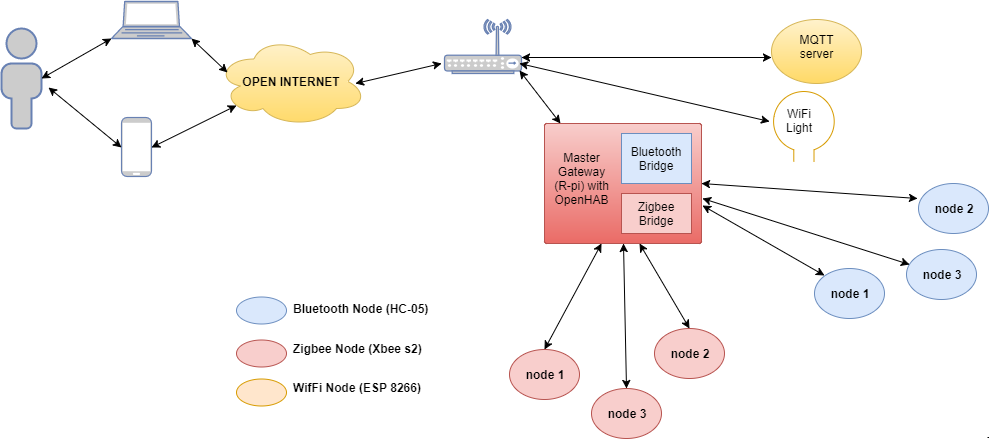
\includegraphics[scale=0.4]{images/architecture_new.png}
\label{fig:1}
\caption{Proposed System Architecture}
\end{figure}
The System Architecture is shown in Figure 1. Some sensors that require constant connectivity like the PIR Motion Sensor, Door vibration sensor, etc. are connected to a Zigbee network since Zigbee specification provides for a highly reliable connection. It consumes very low power and provides a data rate that is sufficient for the readings from these sensors. Other sensors like a room-temperature sensor, moisture sensor, etc. that can afford to lose connection once in a while since their readings do not change rapidly are connected to a Bluetooth network which provides a low-power, low-data rate, low-cost solution with slightly unreliable connection. Other sensors like surveillance cameras that demand high data rates are hooked directly to the Wi-Fi network. By grouping sensors into these three networks, we also try to address the problem of interoperability of different smart devices in the market today. 

\subsection{Bluvironment}
Bluvironment is a Bluetooth based environment monitoring node. It contains DHT22 temperature and humidity sensors and MQ-2 Gas level sensors for sensing combustible gases like LPG, Butane, and Methane. The sensor node is powered by a 2500 18650 Li-Ion battery and contains an HC-05 Bluetooth module for wireless connectivity. The sensor node runs on an Atmega 8 micro-controller clocked at 16 MHz. The sensor node is directly paired with the Bluetooth bridge on the Master Gateway. The sensor sends an environment parameter whenever a change is registered. Otherwise, it keeps its radio turned off to save power. Figure 2 shows the environment monitoring node that is Bluvironment, which works over Bluetooth.
\begin{figure}
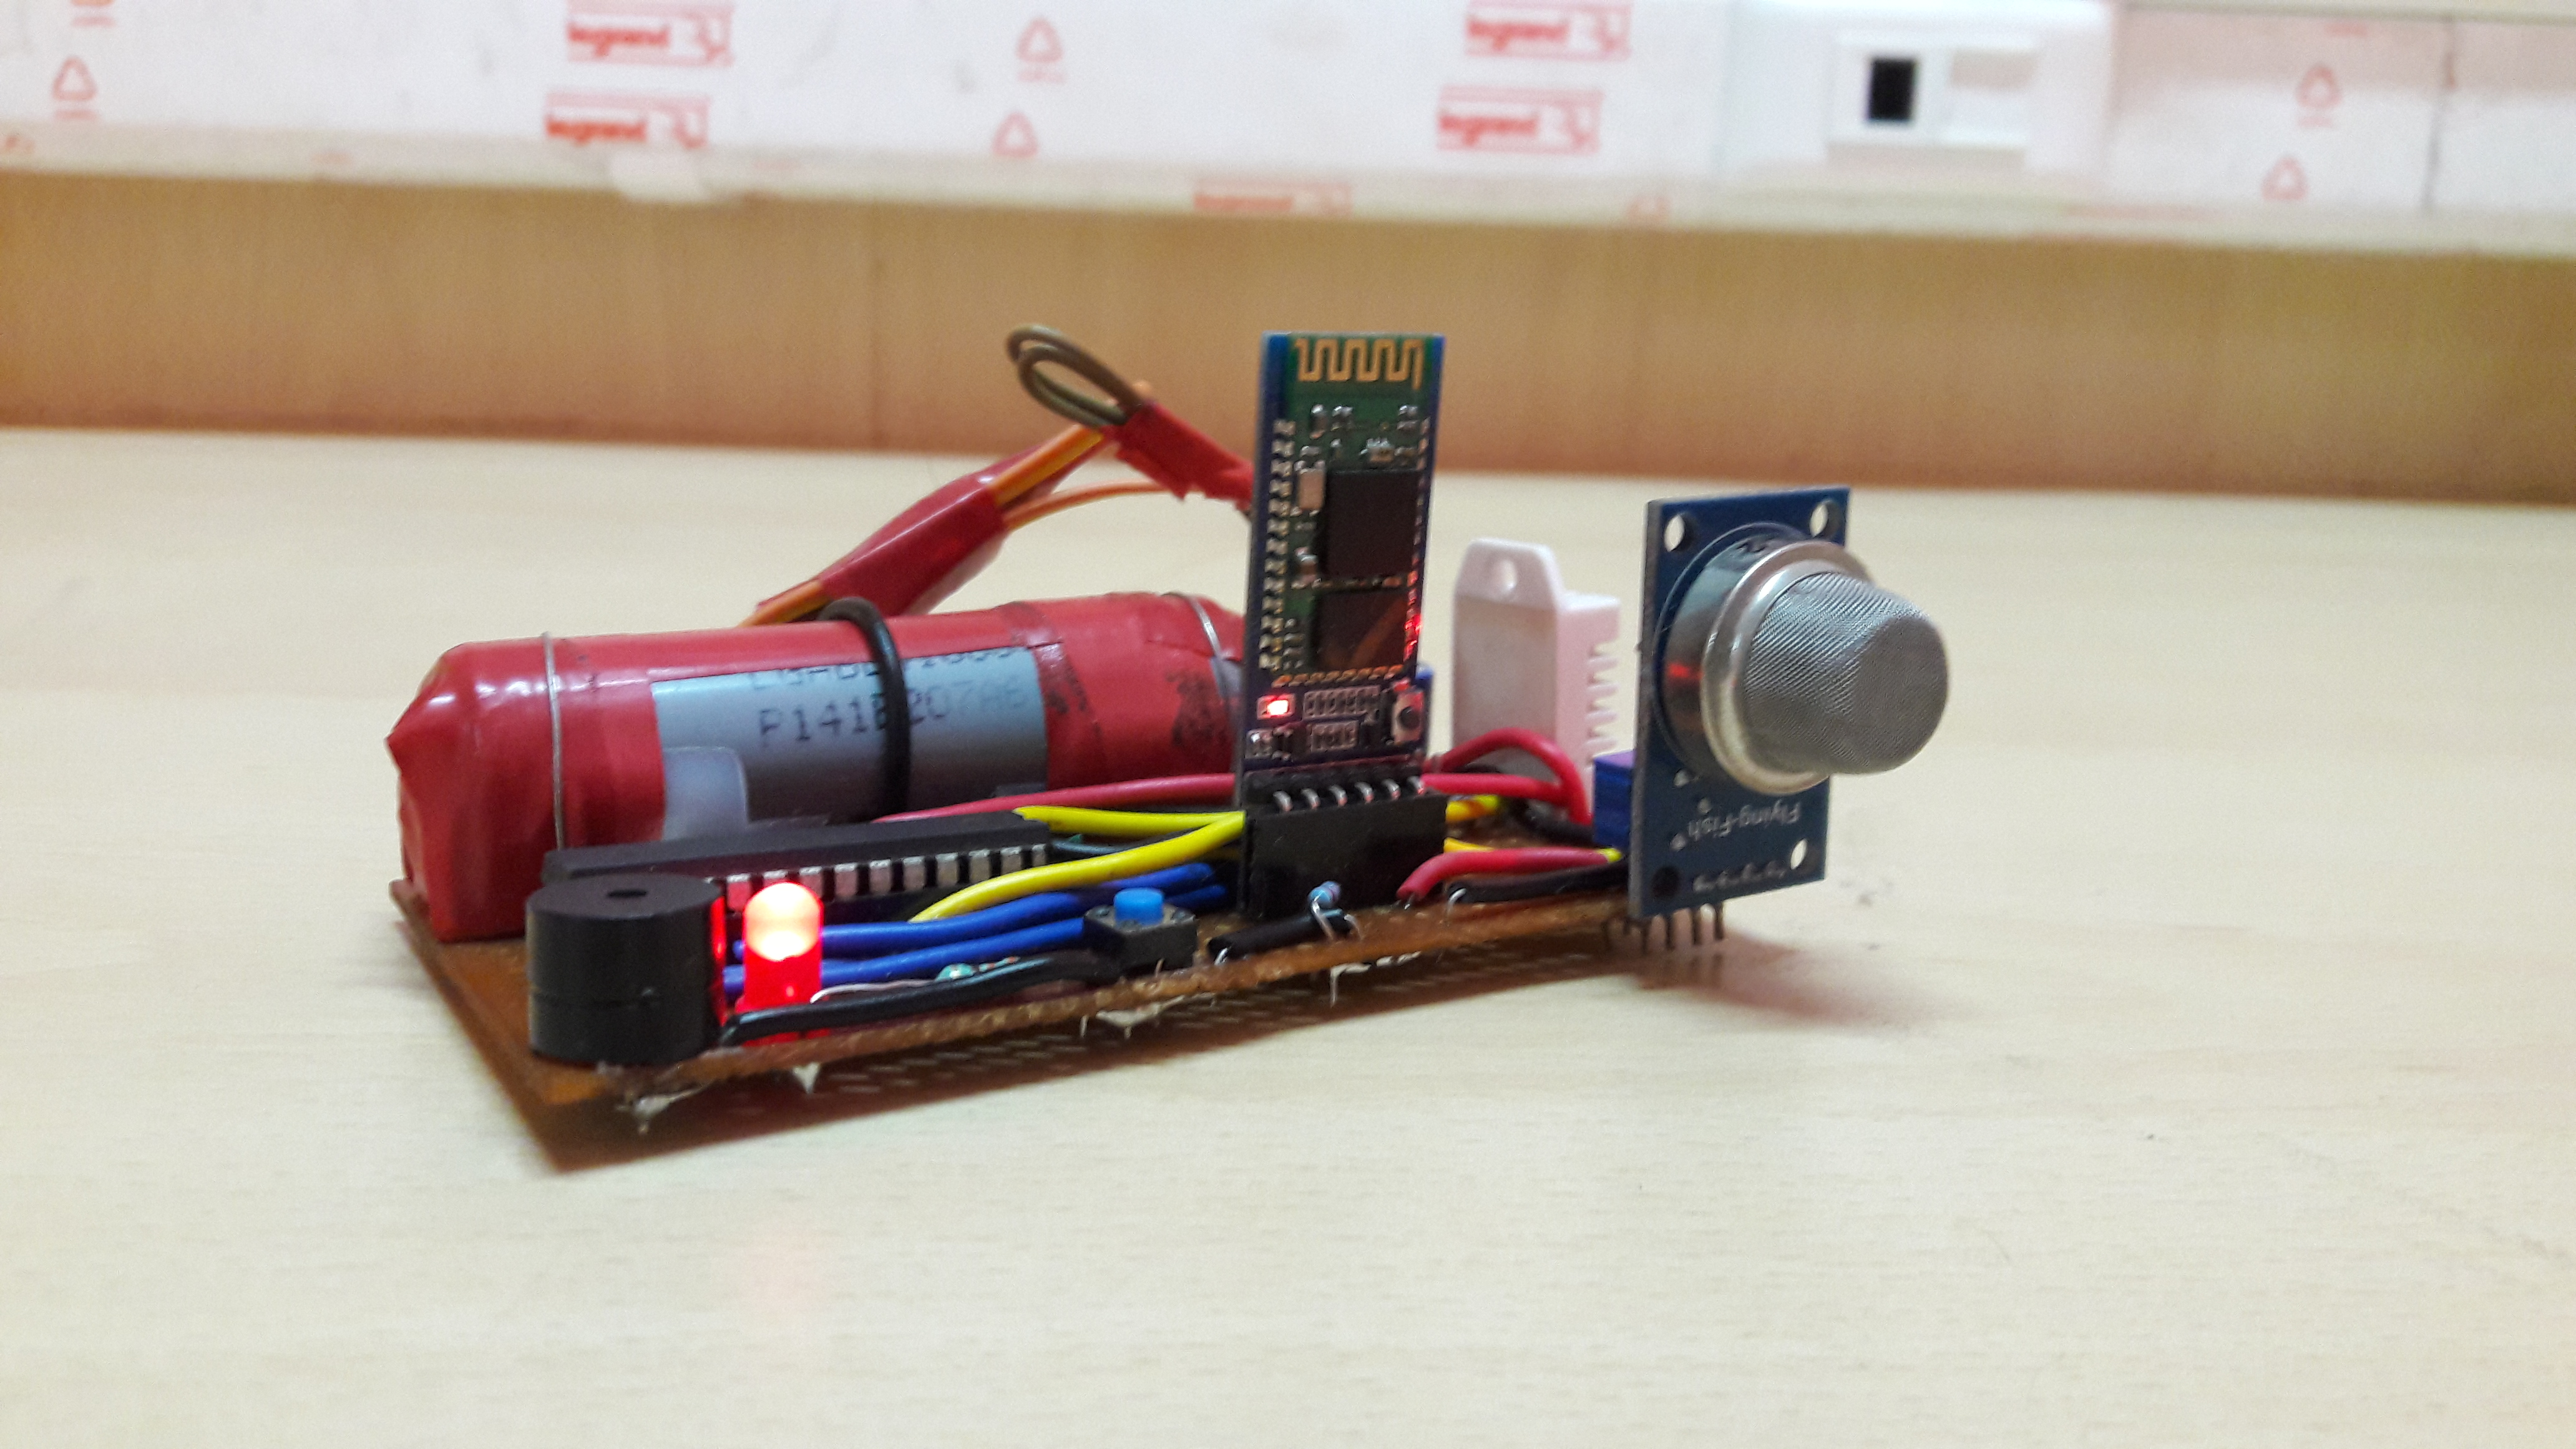
\includegraphics[scale=0.08]{images/environment_monitoring.jpg}
\label{fig:2}
\caption{Bluvironment: Environment Monitoring Node}
\end{figure}

\subsection{Beehealth}
Beehealth is a health monitoring device that tracks movement, heart rate, and body temperature. A digital motion detector - consisting of a 3-axis accelerometer and a 3-axis gyroscope, is mounted with a heart rate monitor and a body temperature sensor. The readings from the array of sensors are read simultaneously in an Atmega328 low-power microcontroller via an I2C interface. The Beehealth micro-controller is attached to an XBee 2.0 Radio device responsible for transmitting cumulative sensor data to another XBee 2.0 Radio linked to the central hub. Beehealth draws power from a rechargeable 1000 mAh Li-Polymer battery. Figure 3 shows the implementation of Beehealth - an elderly monitoring wearable device.

\begin{figure}
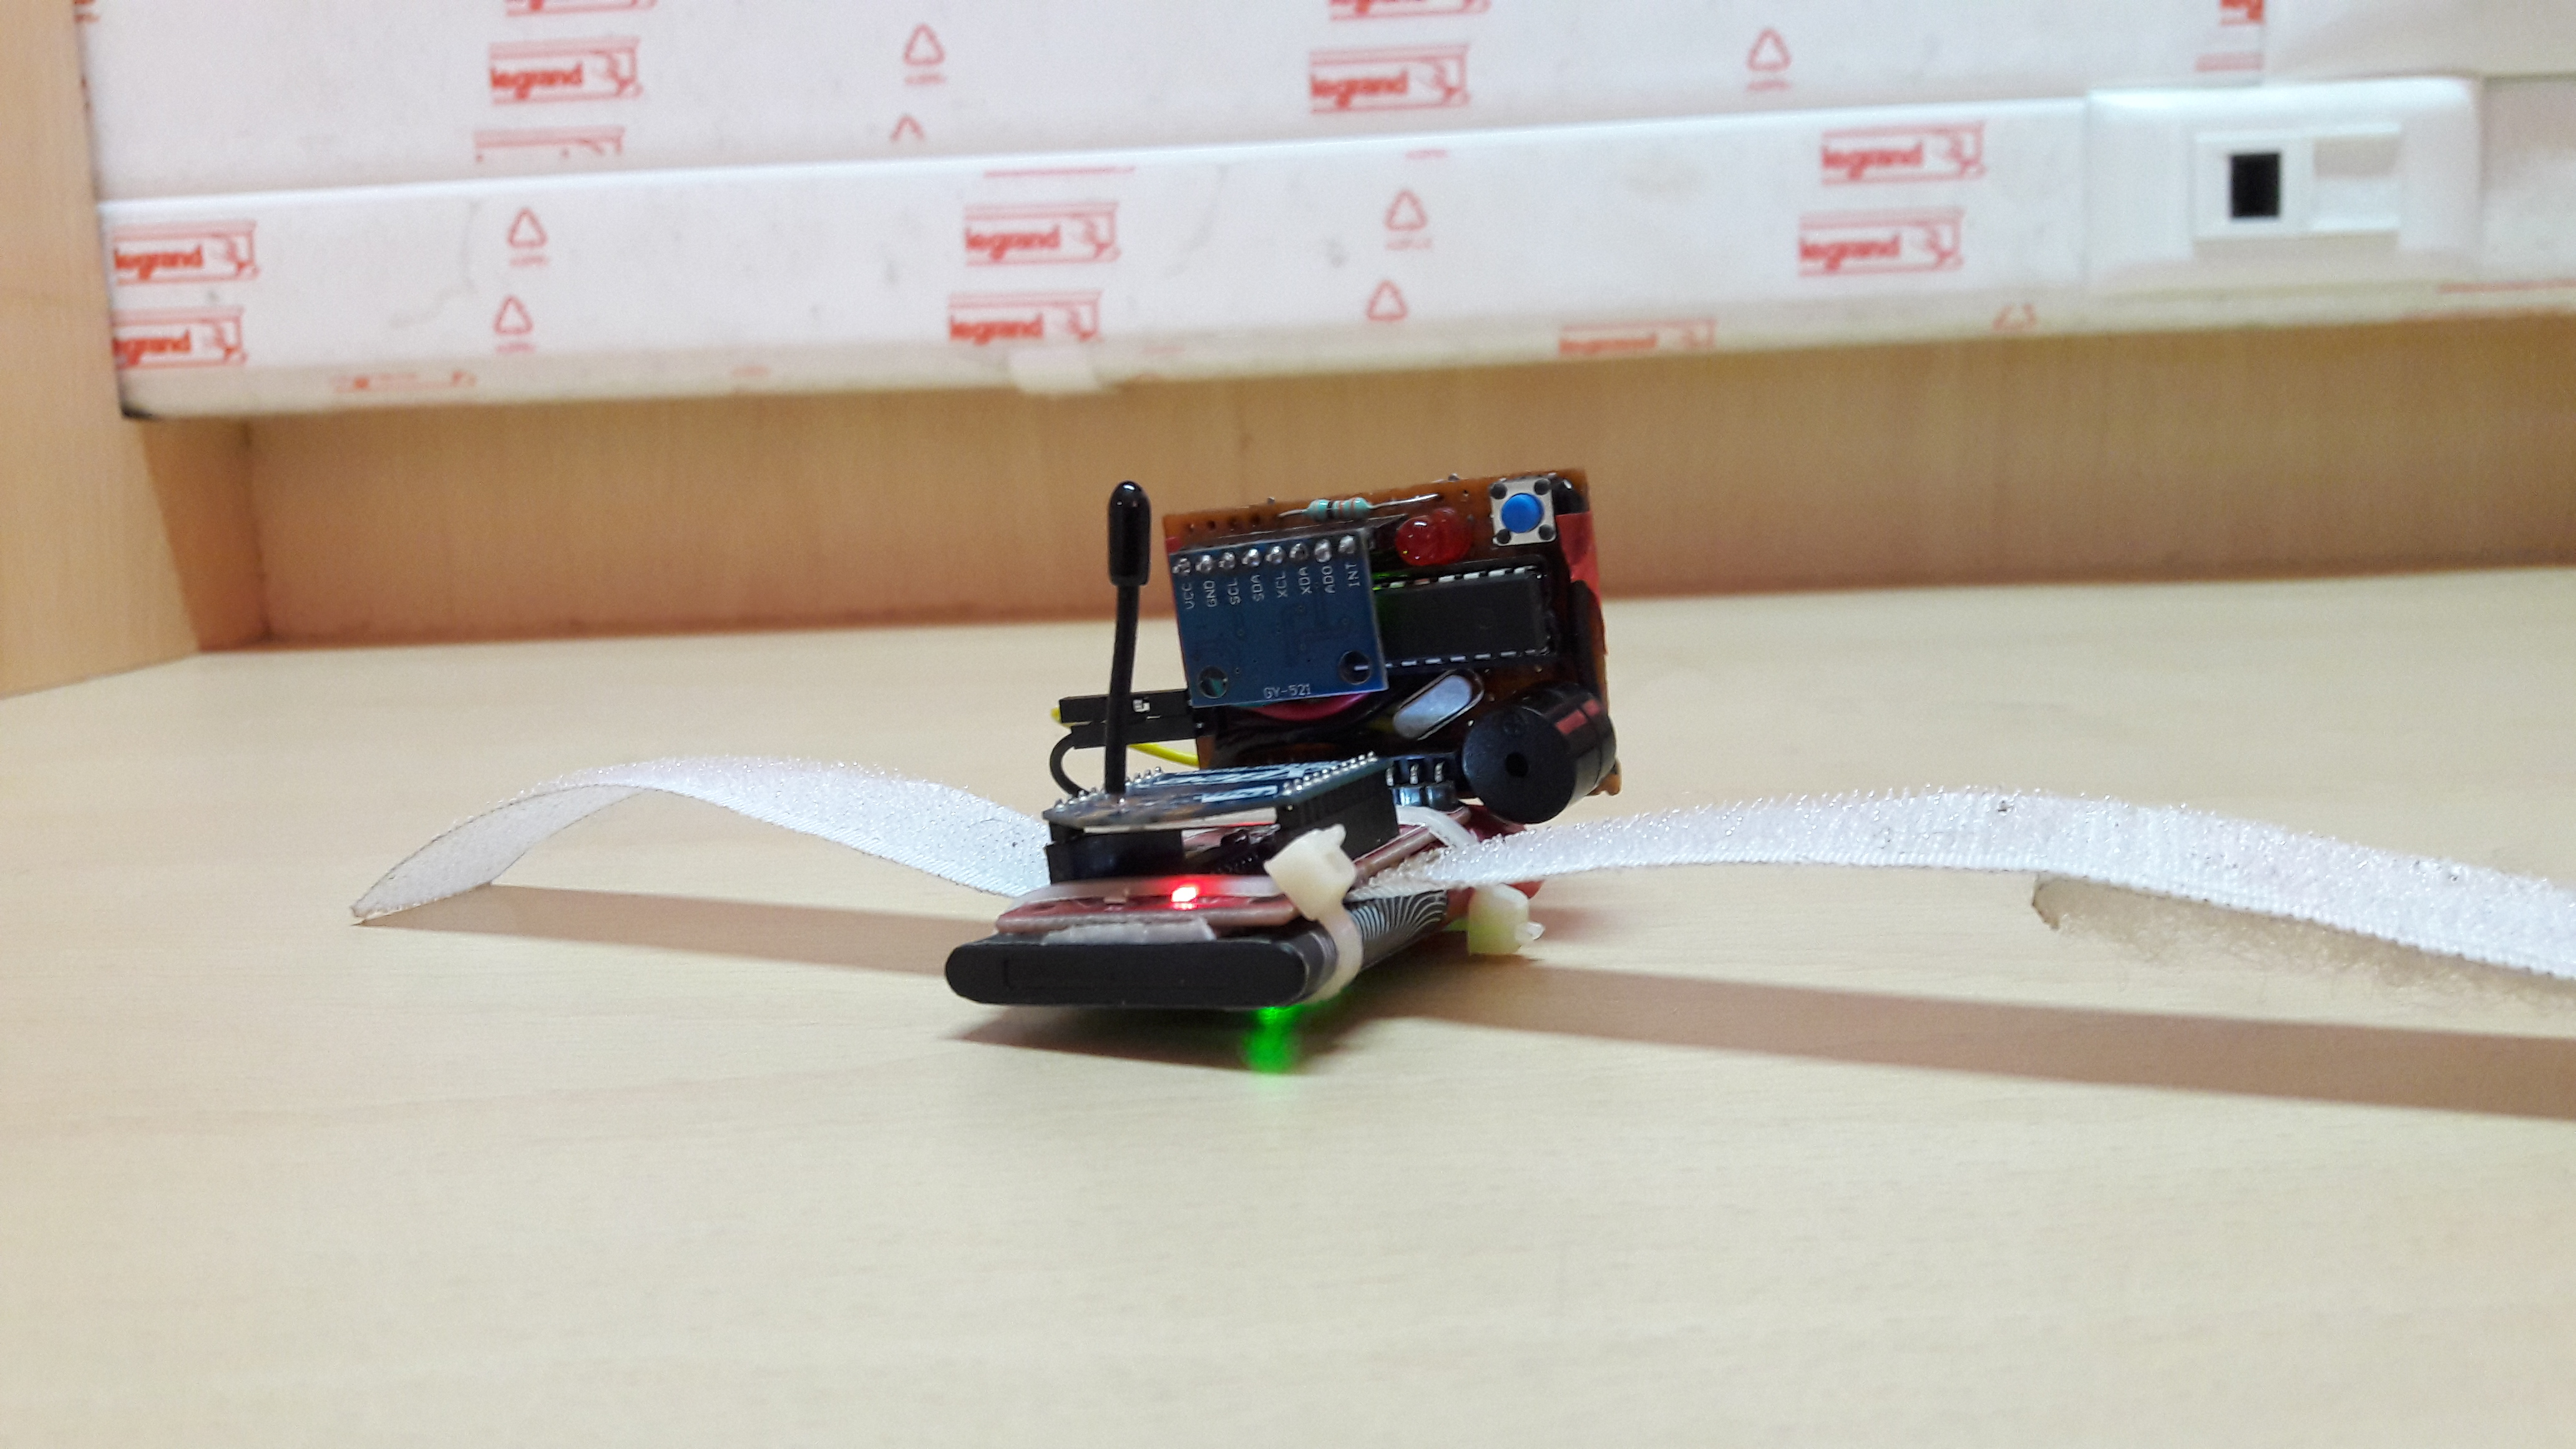
\includegraphics[scale=0.08]{images/elderly_monitoring.jpg}
\label{fig:3}
\caption{Beehealth: Health Monitoring Node}
\end{figure}

\begin{itemize}
\item \textbf{Micro-controller}
Atmega328 micro-controller was used at the heart of the wearable device. The chip contains a programmable flash memory of 32 Kb, which was large enough to accommodate the entire code. It was clocked with a 16 MHz crystal oscillator and programmed using the In-System-Programming interface with the standard USBasp programmer.

\item \textbf{MPU6050 Digital Motion Sensor}
The detector InvenSense MPU-6050 features a MEMS accelerometer and a single chip MEMS gyro. It is very reliable because, for each channel, this includes 16-bit analog hardware for digital conversion. Simultaneously, it captures the X, Y, and Z channels. The sensor uses the I2C-bus to interface with the Arduino.

\item \textbf{Heart Rate Sensor}
A pulse sensor which incorporates a basic optical heart rate sensor with an amplification and noise cancellation circuit to make accurate pulse data easy to obtain. Also, it receives power with just 4 mA current drawn at 5V, so it is great for mobile network-based applications.

\item \textbf{Body Temperature Sensor}
LM35 was used to measure body temperature.

\item \textbf{XBee 2.0 Radio Module}
An XBee Radio configured at 9600 baud rate was used at the wearable device. Another XBee configured as a coordinator was used at the hub. Both XBees were operating within a single Personal Area Network. We configured the destination address of the XBee at the wearable device as the source address of the coordinator. Digi XCTU terminal Software was used to configure the XBees.

\item \textbf{Battery}
800 mAh Li-Polymer 3.7 battery is used. It has a charge time of 1.5 hours and can power the wearable device for 24 to 30 hours. 
\end{itemize}

\subsubsection{Fall Detection - Data Collection}
Acceleration data was collected from an oldage home, 'Chiranthana' in Surathkal, Mangalore. Ten elderly persons were surveyed, and 8 were selected for data collection based on several factors such as the number of activities performed, physical and medical conditions. From the collected data, we identified 8 AODLs (Activities of Daily Living) and the details are as follows:
\begin{itemize}
\item Eating
\item Yoga 
\item Reading
\item Writing
\item Chess
\item Walking
\item Jogging
\item Idle.
\end{itemize}

Therefore, our data set is classified into nine classes (including fall). 
We logged each sample to a file along with a tag representing one of the above 8 activities that the person was performing. To collect the fall data, we asked volunteers to mimic a natural fall in different ways, and we logged the resulting data with a "fall" tag. Overall, we collected data for approximately 2 hours, from each person amounting to about 70,000 samples in total for eight persons. 

\subsubsection{Fall Detection Algorithm}
Most of the existing solutions rely on either of the two techniques, i.e., threshold-based and machine learning-based. We compared both the techniques for accuracy, performance, and robustness. 
\begin{enumerate}

\vspace{15pt}
\begin{figure}[h!]
\label{Threshold Detection}
\centering
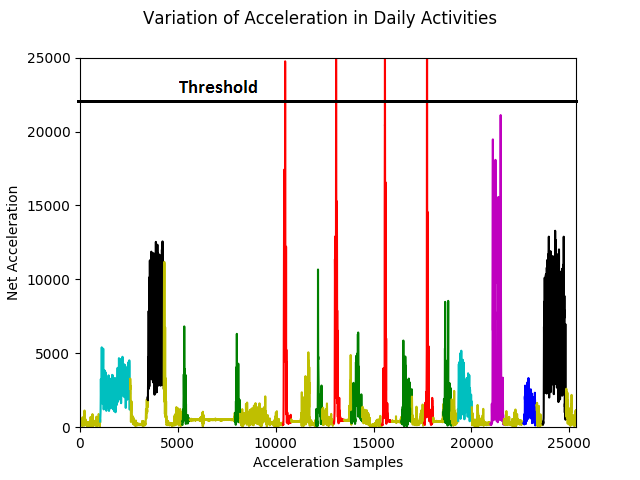
\includegraphics[scale = 0.65]{images/ThresholdSelection}
\label{fig:4}
\centering
\caption{Threshold Detection}
\end{figure}
\vspace{15pt}

\item \textbf{Threshold-based detection}
Our first observation with the collected movement data of the volunteers was - the net acceleration for all activities, except fall, was well below a threshold net acceleration value. Figure 4 shows the threshold-based method for fall detection.

When lower threshold values are selected, more false-positive results are detected whereas, when higher threshold values are selected, relatively less amount of false-negative results are detected. False-negative detection can have more disastrous consequences compared to a false positive detection - consider a situation when a person falls, but the Fall Detection device does not report the fall, leading to severe repercussions. Therefore, our selection of relatively lower threshold value minimized false-negative detection at the cost of a few false positive detections. To obtain an optimum threshold value, we plotted threshold values against false positive and false negative detection.

The method is computationally inexpensive and is widely suitable for wearable devices where computational resources such as bandwidth and power are major constraints. Once we determine a sufficiently accurate threshold value from the collected movement data, we can easily perform the fall detection at Beehealth itself instead of streaming sensor data to the central hub and then detecting fall. Therefore, saving data transfer bandwidth and limited power of Beehealth.

\item \textbf{Neural Network}
Although the threshold-based fall detection method can provide sufficiently accurate results in most real-world situations, a well-constructed machine learning algorithm proves to be more accurate by further minimizing the false-positive results. Machine learning can bring out the patterns in data collected by movement sensors along with the heart rate and body temperature sensors.

We used Neural Networks as they are the most commonly used algorithms for pattern recognition for their inherent ability to generalize, analyze, and to respond to unexpected inputs variations. In the process of training, neurons are made to learn to recognize numerous specific variations in patterns and whether it is better to fire when a particular pattern is received. If a pattern is received during the time of execution stage that is not associated with a particular output, the neuron might select the output, which will correspond to a particular pattern from the set of given patterns that it has been taught of, that will be least different from the input.

To design a neural network for fall detection and get robust fall detection compared to the threshold-based fall detection method, it is paramount to build a relevant and thoroughgoing feature set from the collected data set. We further look into the set of features derived from the collected movement data in this section.\\

\textbf{Feature Extraction}:
We form all data points by extracting features from a window of consecutive net acceleration values in the collected movement data encompassing all eight classes of AODLs and fall. We selected the window size as 300 since most of the AODLs lasted for around 300 points of net acceleration. The features extracted from the collected movement data are as follows:

%\vspace{15pt}
\begin{figure}[h!]
\label{Feature maps:1}
\centering
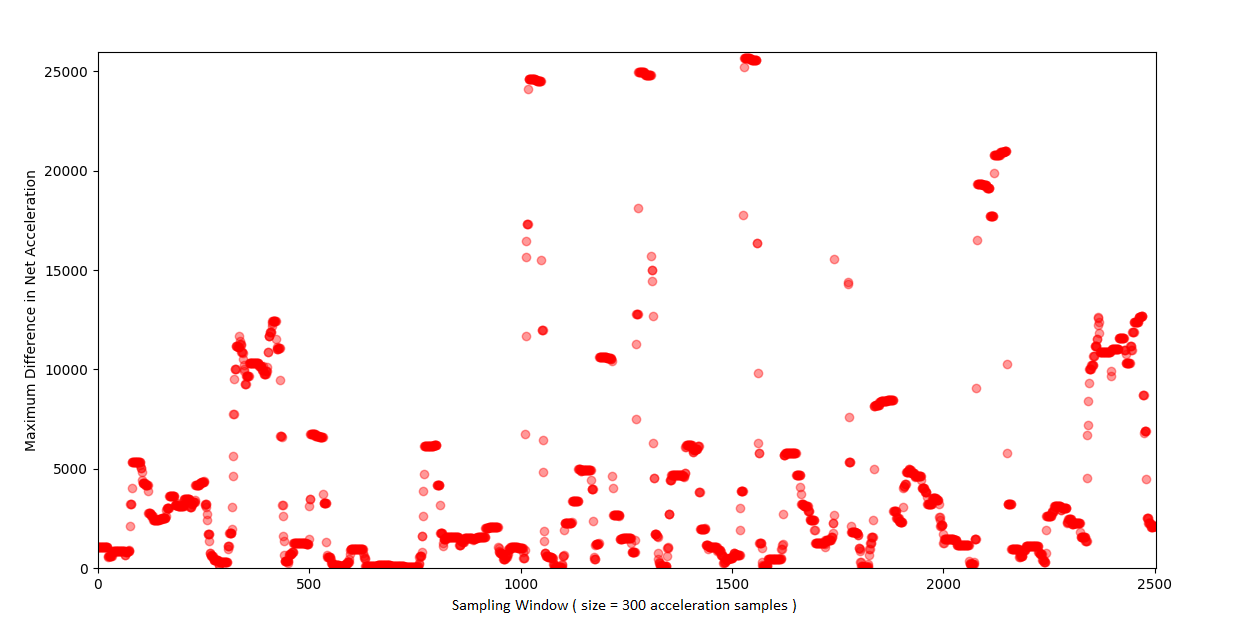
\includegraphics[scale = 0.40]{images/max_difff}
\centering
\label{fig:5}
\caption{Maximum Net Acceleration Difference}
\end{figure}
%\vspace{15pt}

\begin{itemize}
\item \textbf{Maximum Difference}: By investigating the collected data, we recognized that the maximum difference between two consecutive net acceleration values within a window is higher in the event of a fall compared to the same in case of other AODLs like idle, walking, vibrations, etc. Shown in Figure 5.

%\vspace{15pt}
\begin{figure}[h!]
\label{Feature maps:2}
\centering
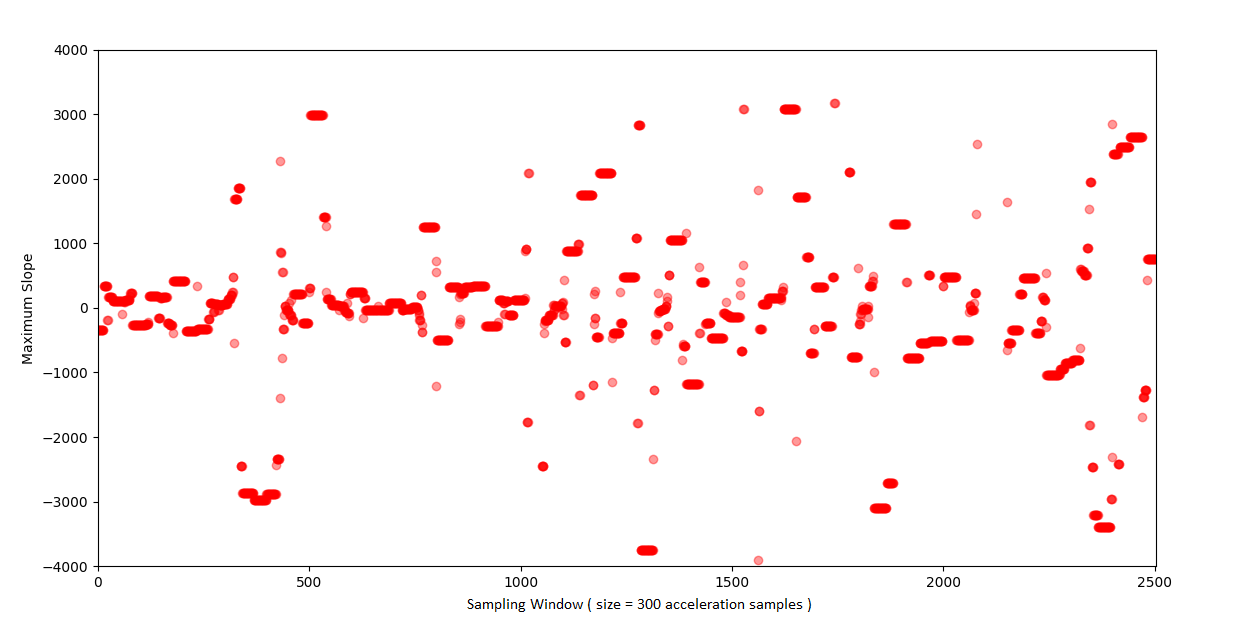
\includegraphics[scale = 0.40]{images/max_slope}
\label{fig:6}
\centering
\caption{Maximum Slope}
\end{figure}
%\vspace{15pt}

\item \textbf{Maximum Slope}: In the event of a fall, we noticed a sudden increase in net acceleration, which further implies sheer slope. Thus, the maximum slope of a consecutive net acceleration window is always higher in case of a fall compared to the same in case of all other AODLs. Details are shown in Figure 6.

%\vspace{15pt}
\begin{figure}[h!]
\label{Feature maps:3}
\centering
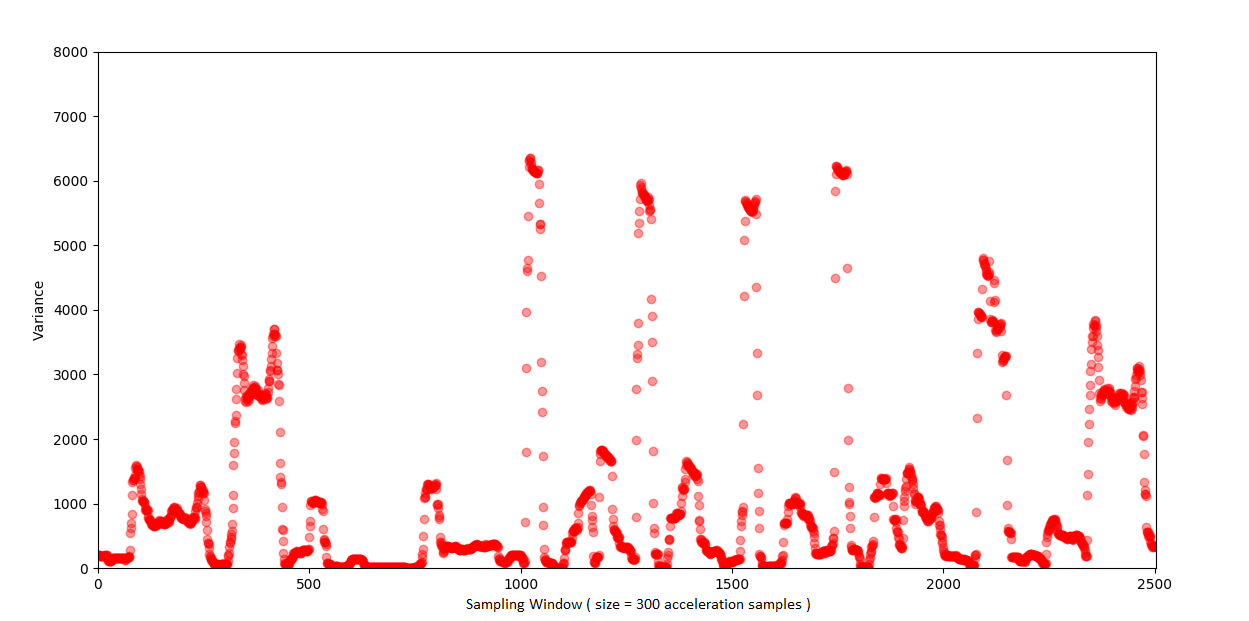
\includegraphics[scale = 0.40]{images/variance}
\label{fig:7}
\centering
\caption{Variance}
\end{figure}
%\vspace{15pt}

%\vspace{15pt}
\begin{figure}[h!]
\label{Feature maps:4}
\centering
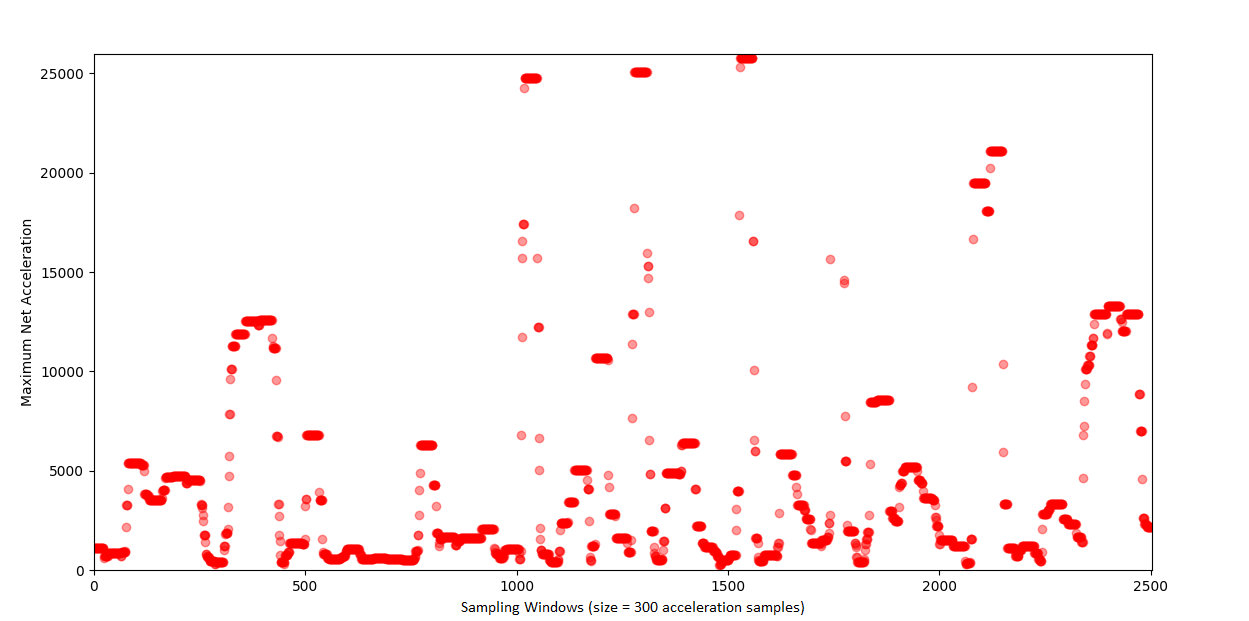
\includegraphics[scale = 0.40]{images/max_acc}
\label{fig:8}
\centering
\caption{Maximum Net Acceleration}
\end{figure}
%\vspace{15pt}

\item \textbf{Variance}: AODLs like walking, running, or vibrations are a collection of repeating patterns, i.e., the net acceleration in such AODLs oscillates around a mean position throughout the activity - resulting in low variance within a consecutive net acceleration window. However, in the event of a fall, which is characterized by a sudden increase in net acceleration, the mean acceleration of the net acceleration window is high. Although, most of the neighboring points are far away from the mean of the window, therefore, the variance of the consecutive net acceleration window is high, as shown in Figure 7. 

\item \textbf{Maximum Acceleration}: In the case of a fall, the maximum acceleration within a consecutive net acceleration window is found to be higher than in other AODLs like eating, chess, reading which involves little too sparse movement. In simple terms, this feature is the incorporation of a threshold-based fall detection method in the neural network as shown in Figure 8. \\

\end{itemize}

\textbf{Training parameters}: We used the following parameters for the neural network.

\begin{itemize}
\item Input Layer - 4 (Number of features)
\item Hidden Layers - 1 (size = 2)
\item Output Layer - 1 
\item Activation function for Hidden layer - Logistic Sigmoid Function
\item Solver for weight optimization - lbfgs
\item Learning Rate (alpha) - 0.0001
\item Learning Rate Schedule - Constant Learning Rate
\item Maximum Number of Iterations - 200.

\end{itemize}
\end{enumerate}

\begin{figure}[H]
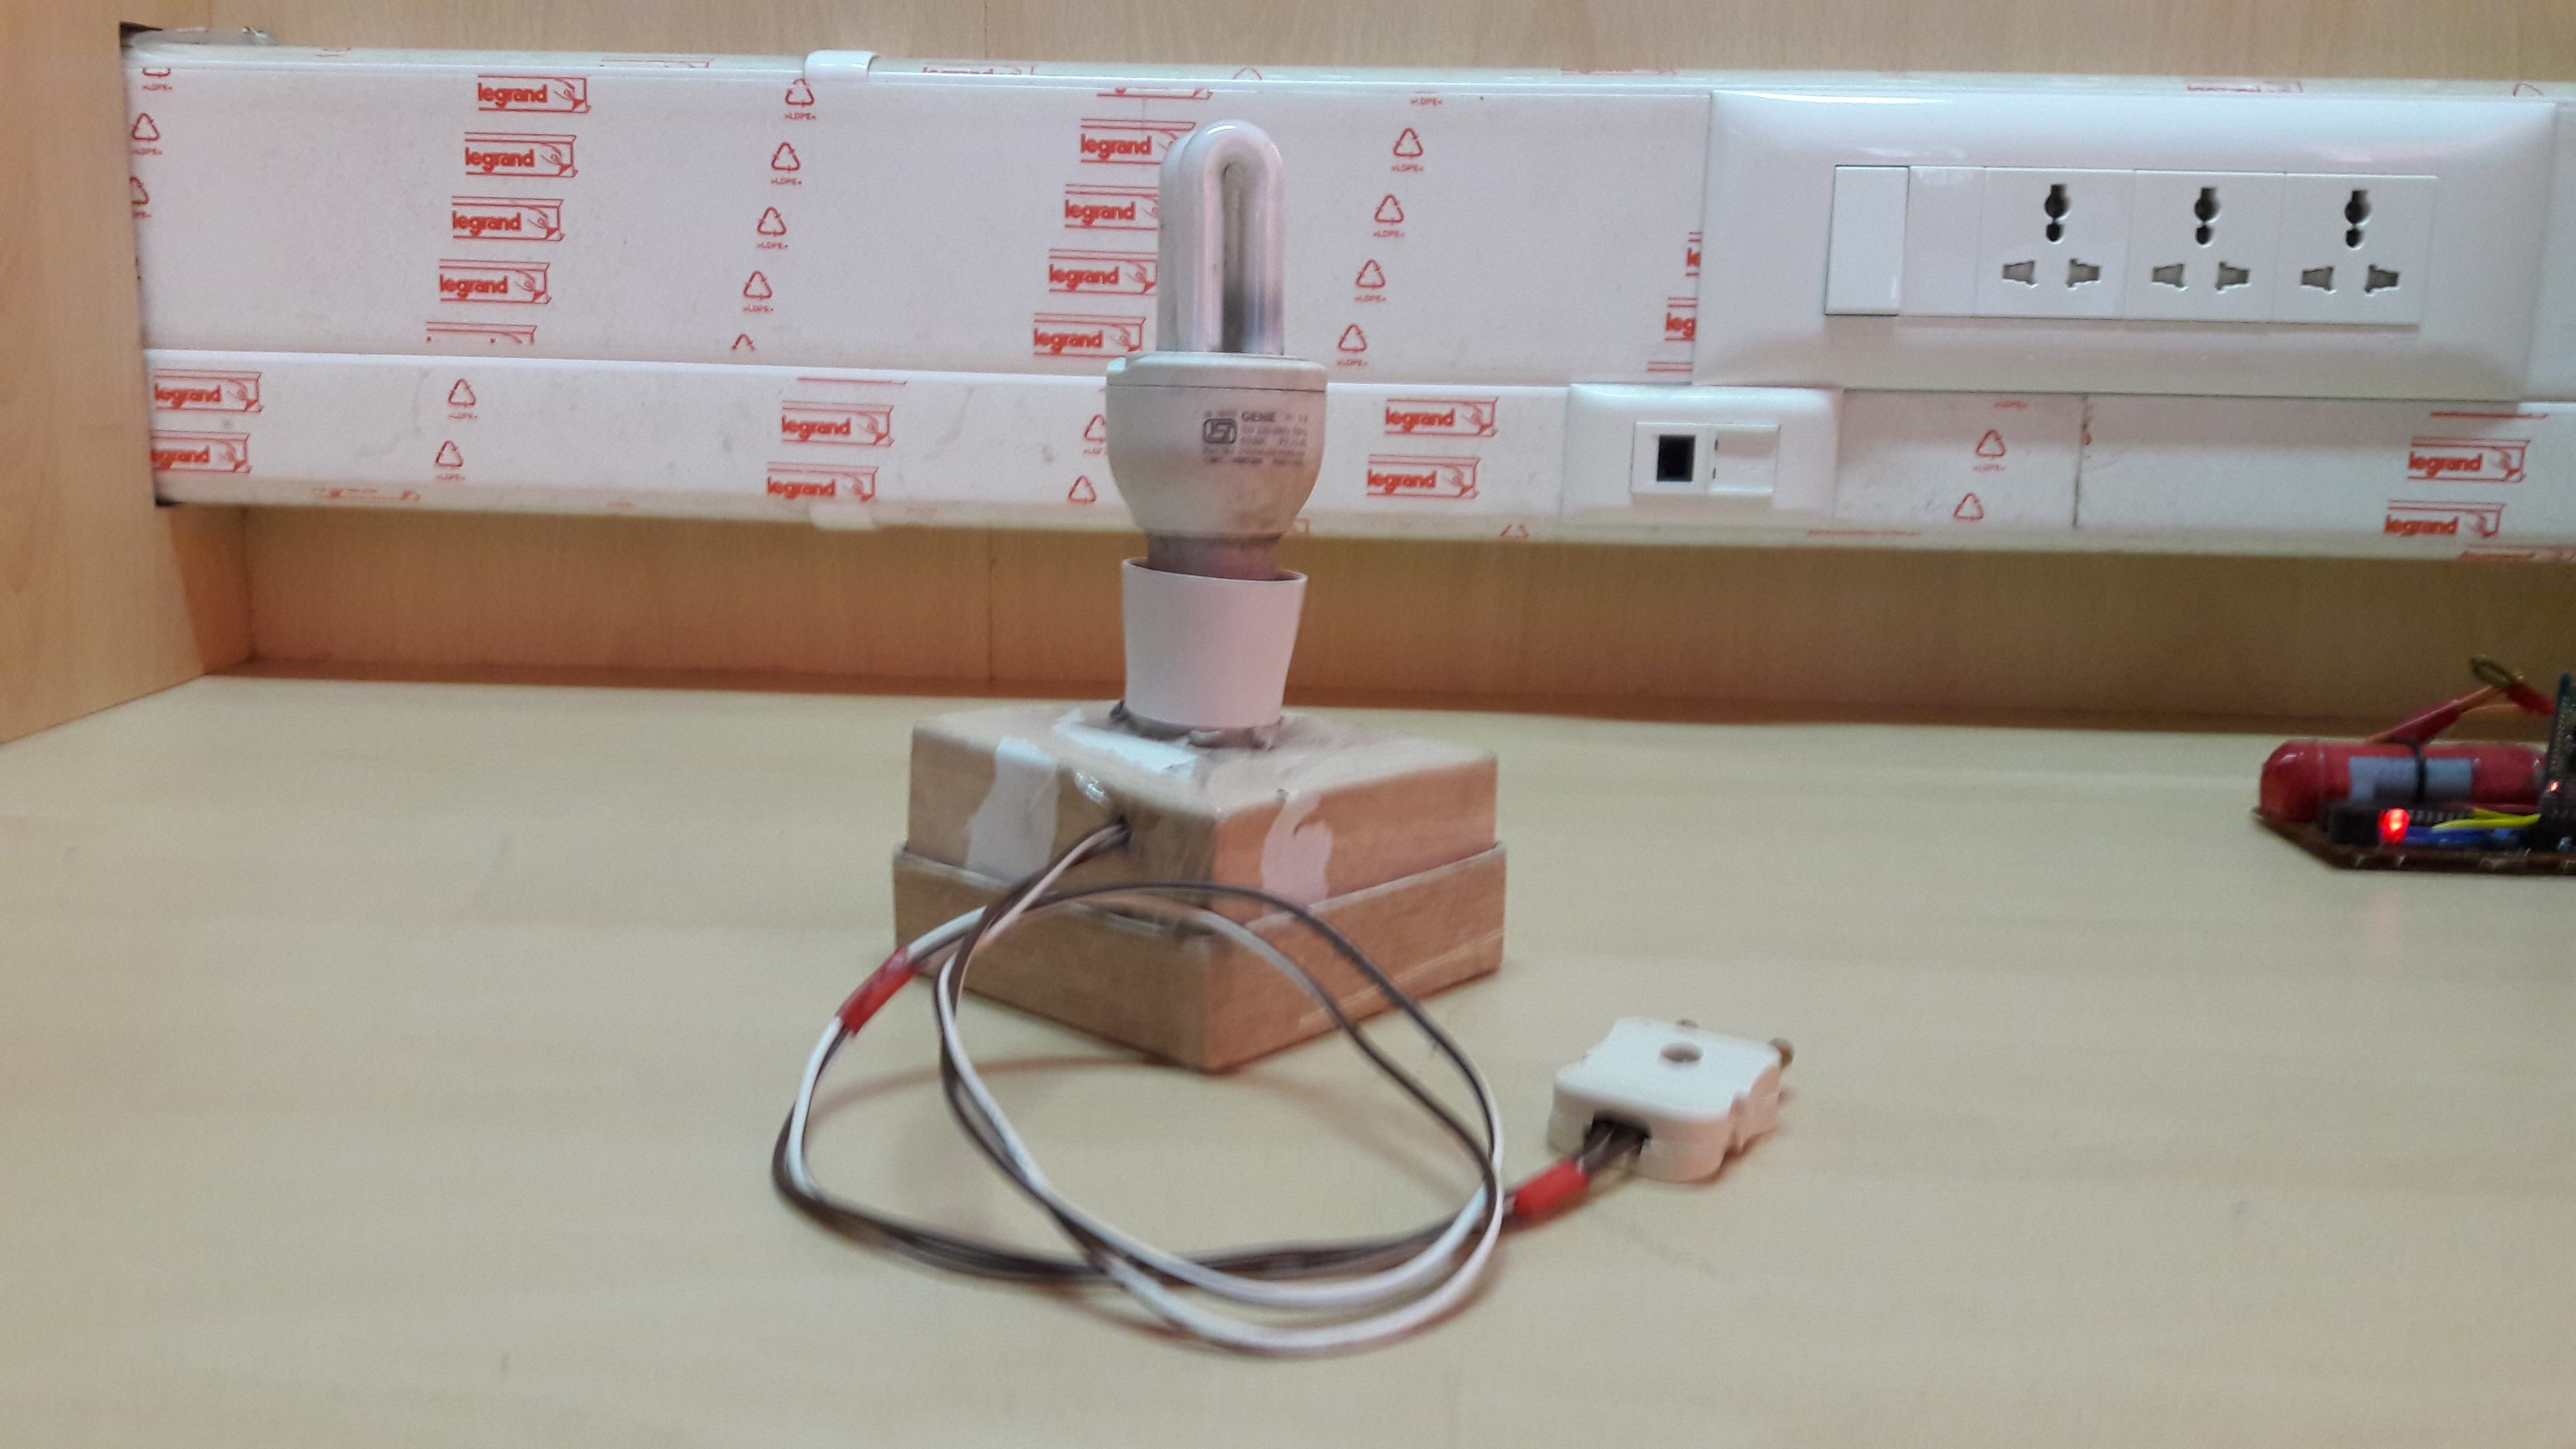
\includegraphics[scale=0.08]{images/wifi_light.jpg}
\label{fig:9}
\caption{Wi-Fi light}
\end{figure}

\subsection{Wi-Fi Light}
An ESP8266 based light with Wi-Fi capability uses the MQTT publish-subscribe protocol. It directly connects to the available Wi-Fi network and subscribes to an appropriate topic (ex: Living Room/Light) and listens for any message published on that topic. Whenever the user commands OpenHAB to turn the light ON/OFF, the message is published on that particular topic by the Master Gateway. Upon receiving this message, the Wi-Fi light can turn ON/OFF. To switch the 220 V AC circuit, the module makes use of a 12 V relay. No battery is required in this application as the power for ESP, and the relay can be drawn from the 220 AC Mains using a step-down transformer and a bridge rectifier. Figure 9 shows the implemented Wi-Fi bulb.


\subsection{Master Gateway}
The central hub for the home automation system is a Raspberry Pi. The central hub, connected to the internet, is powered by OpenHAB - an open-source Home Automation Framework which provides a user-friendly interactive interface in the form of Web, Android, and iOS application. Through device-specific bindings, OpenHAB can communicate with most smart devices available in the market, making it universal and extensible. The Master Gateway components are listed below.

\begin{itemize}
\item \textbf{Raspberry Pi}
Raspberry Pi 3 was used as the central Hub. It was interfaced with an XBee Radio Module through a serial interface. The hub was connected to the internet. 
\item \textbf{OpenHAB}
OpenHAB is a widely used home automation framework. We used it to power the central hub. It provides Zigbee bindings that can easily interface with any Zigbee device. 
\item \textbf{Speaker}
The gateway is connected to a speaker for multimedia and voice feedback. 
\item \textbf{Bluetooth Bridge}
An HC-05 module acts as a Bluetooth Bridge enabling the Master Gateway to communicate with the Bluetooth devices in the network. 
\item \textbf{Zigbee Bridge}
An XBee s2 module acts as a Zigbee Bridge enabling the Master Gateway to communicate with the Zigbee devices in the network. Figure 10 shows the gateway of the entire network.
\end{itemize}

\begin{figure}[H]
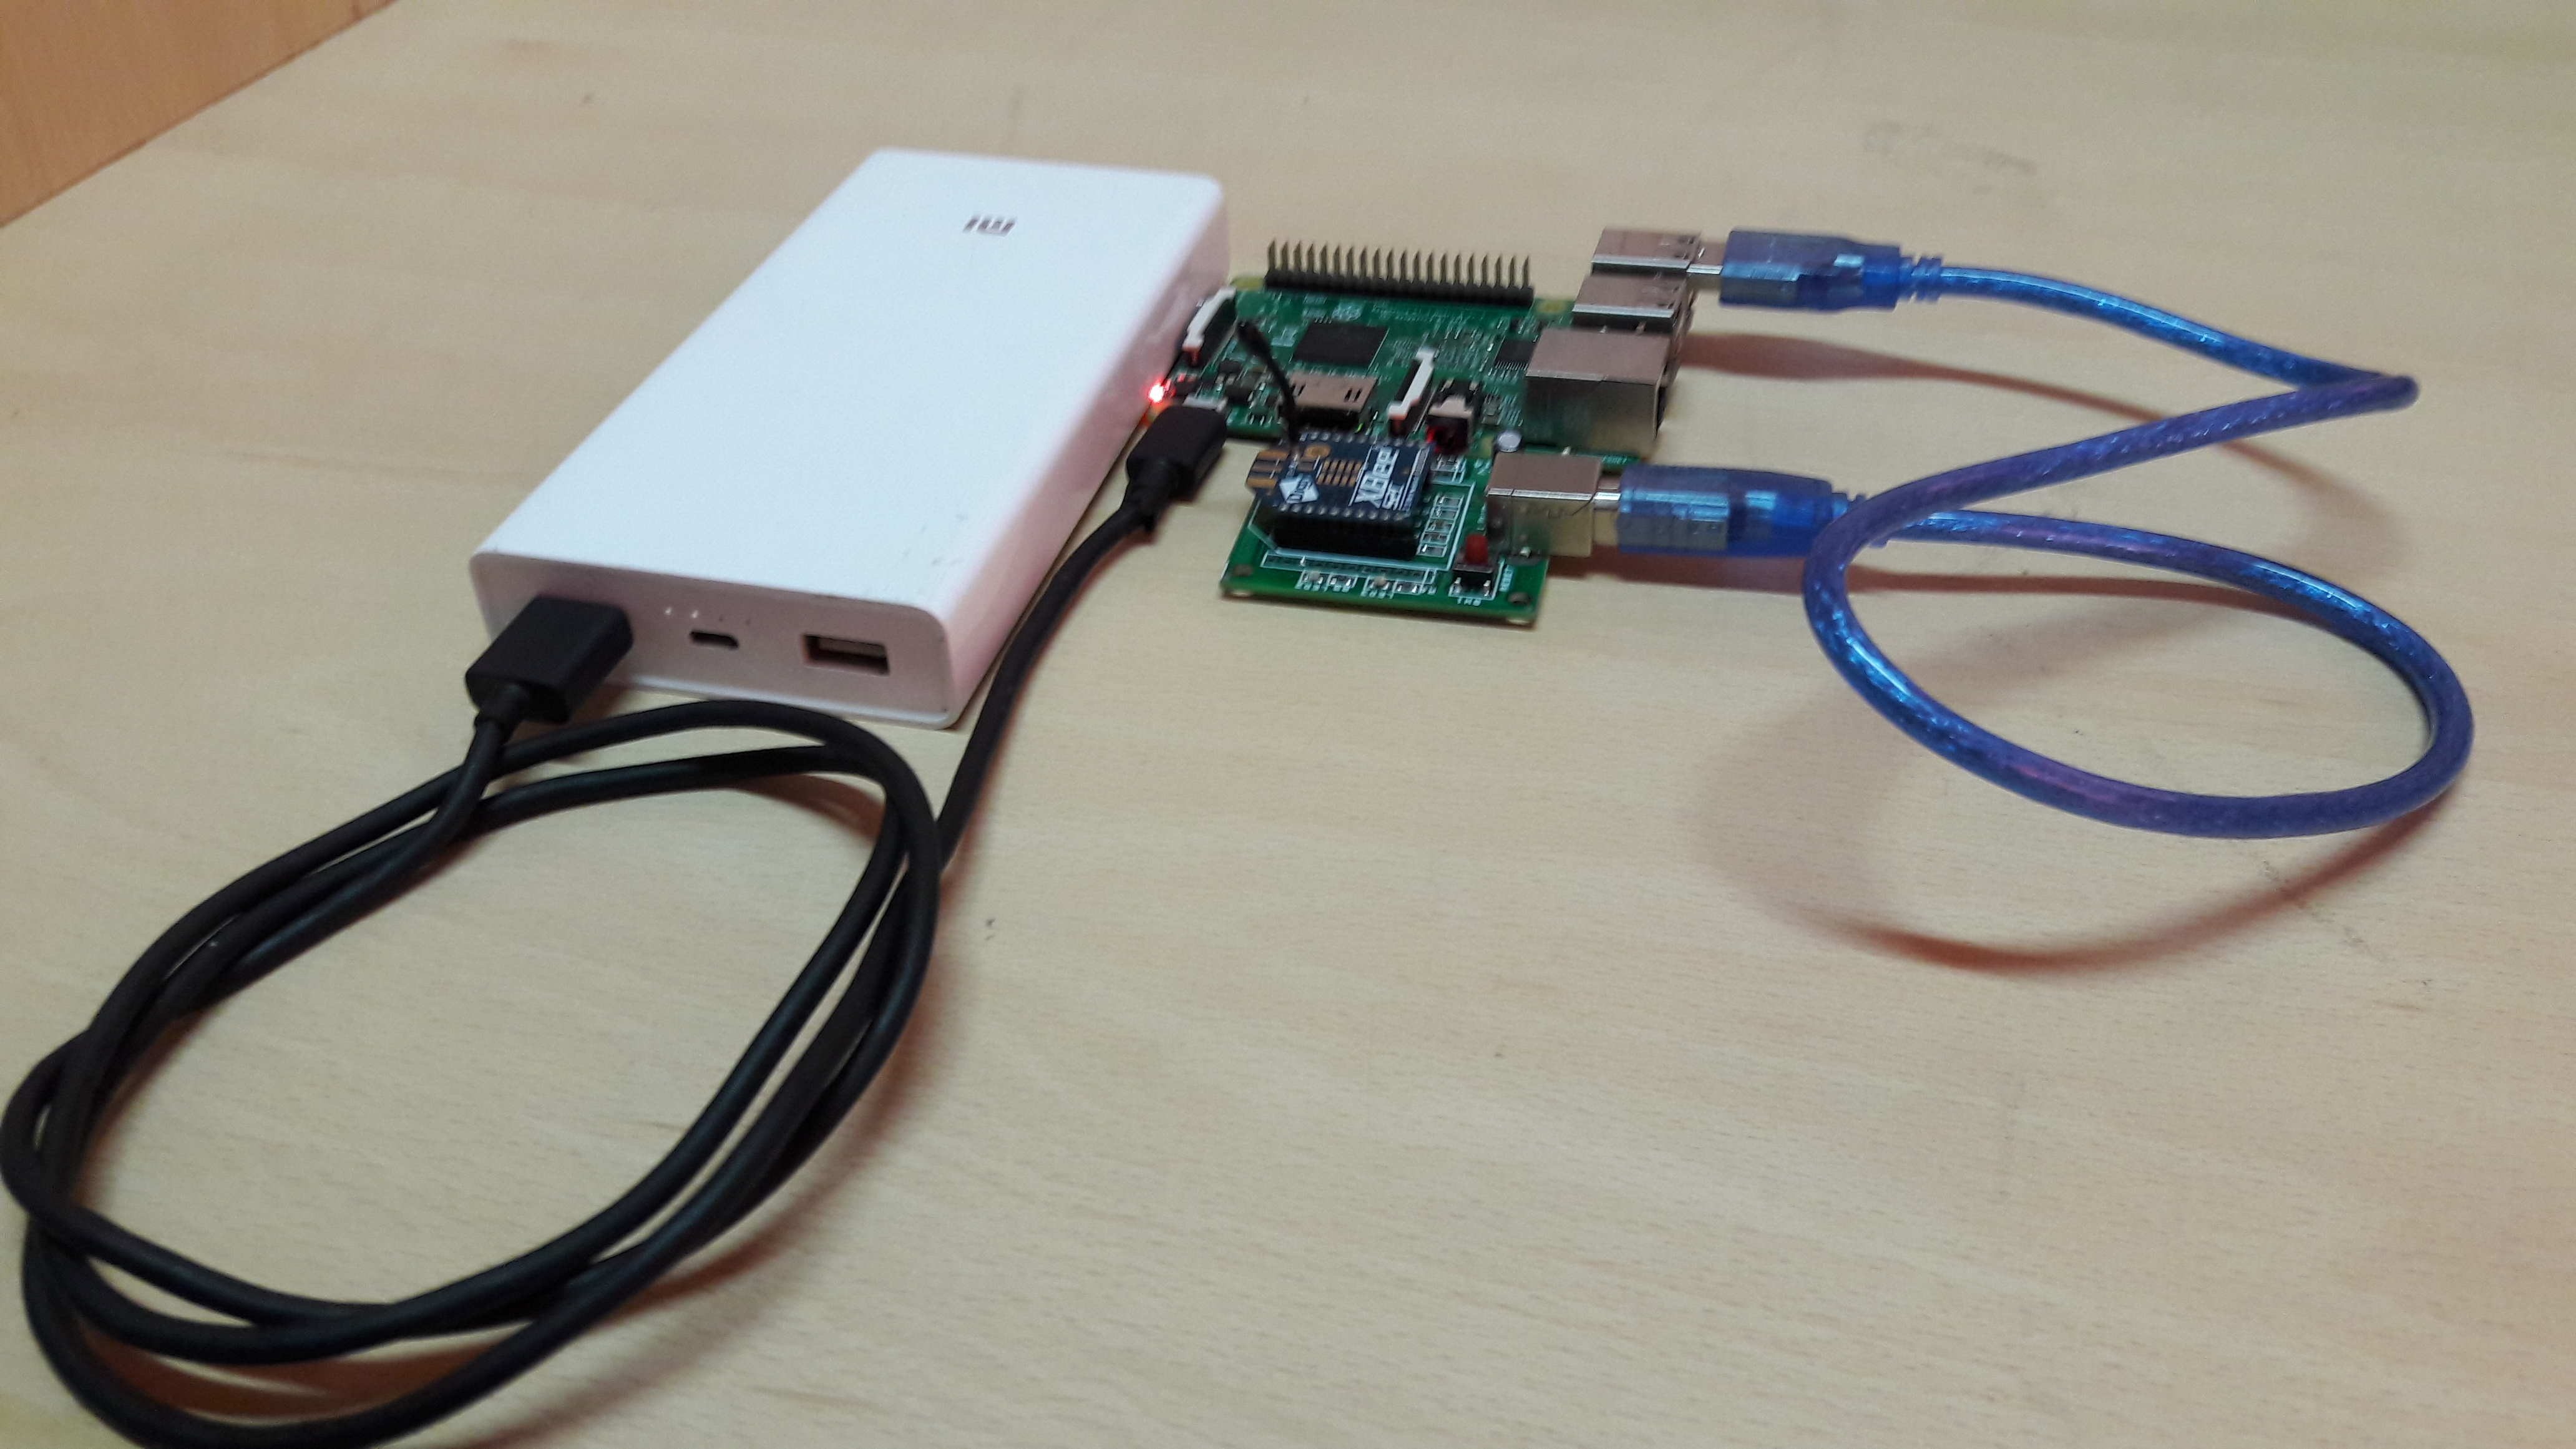
\includegraphics[scale=0.08]{images/gateway.jpg}
\label{fig:10}
\caption{Zigbee gateway}
\end{figure}

%\newpage

\section{Results and Analysis}

\subsection{Evaluation Metrics}

We evaluate the Multi-protocol Smart Home devices on the following metrics.
\begin{itemize}
\item \textbf{Syncing Time} - Syncing time is the average time taken by the Smart Home devices to transmit data to the master gateway. For devices running on chargeable battery, the average syncing time was calculated over a complete discharge cycle, i.e., average syncing time, while the attached power source discharges from 100\% to 0\%. However, in the case of Wi-Fi Light, the syncing time is the delay in operation being actually performed after being initiated by the user. Hence, we measured the delay in 100 power on/off operations and calculated the average of all the measured delays.
\item \textbf{Battery life} - Battery life for Smart Home devices working on the rechargeable battery is the average run time of the device on a full charge. For Bluvironment, we measured the running time over one discharge cycle, whereas for Beehealth, the average running time was measured over 30 discharge cycles.
\item \textbf{Recharging Time} - Recharging time of a device drawing power from a battery is defined as the time taken for the battery to charge from 0\% to 100\%. For Bluvironment, the recharging time was the average over 2 recharges, while for Beehealth we measured the average recharging time as the average of 30 recharges.
\item \textbf{Deployability} - We define deployability of Smart Home devices as the maximum distance between the device and the smart gateway such that the syncing time is not affected. In the ideal case, master gateway and the connected device will be in their respective line of sight, although, in the real-world scenarios, we introduce obstacles such as wall and moving people between the Smart Home device and the master gateway. We calculated the average distance in various real-world scenarios and an ideal case.
\item \textbf{Cost} - Cost of the designed Smart Home devices refers to the sum of all the individual components required to manufacture a working device. These individual components were bought at retail prices; therefore, all these Smart Home devices will cost a bit cheaper if bought at bulk prices.

\end{itemize}

Table 2 shows the Evaluation metrics for different implemented modules. We discuss the performance of different Smart Home devices given below:

\begin{itemize}
    
\item \textbf{Bluvironment} - Bluvironment transmits data relatively slower but provides an excellent battery life, which lasts for around 55-60 days. Excellent battery life, along with deployability of 20 meters, ensures efficiency as well as reliability of Bluvironment when used in real-world scenarios. Smart Homes has a minimal recharging time of 6 hours when compared to the average battery life of around 55 days. With the cost of components amounting to just around Rs. 600, Bluvironment is an affordable home and environment monitoring Smart Home device.

\item \textbf{Beehealth} - Beehealth is an efficient, fast, and reliable health monitoring device with a syncing time less than a second battery life of over a day and deployability of around 100 meters. The full recharge time of Beehealth is also significantly lower than at 1 hour.
The cumulative price of Beehealth’s component sums to Rs. 2000, which is significantly lower compared to the implementation costs in [21, 22]. However, we can reduce the weight and cost of Beehealth can further by optimizing the power consumption of the device, which will allow for a smaller battery.

\item \textbf{Wi-Fi Light} - Wi-Fi light uses MQTT protocol for receiving instructions from the master gateway; thus, syncing time is around 5 seconds. Wi-Fi light has deployability of around 100 meters, allowing a user to install this Smart Home device almost anywhere in the house. Wi-Fi light costing for around Rs. 300 is a remarkably cost-effective solution for appliance control.

\end{itemize}

\begin{table}[H]  
\caption{Evaluation Metrics}
\begin{tabular}{ | m{3cm} | m{2cm}| m{2cm} | m{2cm} | }
\hline
\textbf{Metric} & \textbf{Bluvironment} & \textbf{Beehealth} & \textbf{Wi-Fi Light} \\
\hline    
 1.Syncing Time & 2-3 seconds & less than 1 second & 4-5 seconds \\ 
 \hline
 
2.Battery life & 55-60 days & 24-30 hours & NA \\
  \hline

3.Recharging Time & 6 hours & 1 hour & NA \\
  \hline 

4. Deployability & 20 meters & 100 meters & 50-100 meters \\
\hline

5. Cost & Rs. 600 & Rs. 2000 & Rs. 300 \\
\hline

\end{tabular}
\end{table}



\vspace{10pt}
\textbf{Compatible Platforms:}
\begin{itemize}
\item Desktop/PC :- Web browsers
\item Android :- Android Application
\item iOS :- iOS Application
\end{itemize}

\vspace{10pt}
\textbf{Miscellaneous features:}
\begin{itemize}
\item Real Time Weather Forecast
\item Real Time Astronomical Data
\item On-line Radio 
\item Alarm Notification
\item Voice Feedback
\end{itemize}

\subsection{Fall Detection Results}
In this section, we compare the results obtained from using both the techniques - threshold-based and Neural Network-based.

\begin{itemize}
\item \textbf{Threshold-based Fall Detection}: The method works relatively well under most conditions with a reasonable threshold. It is computationally inexpensive; thus, it can be effectively implemented in a wearable device with limited power and computation. The identification was effective in all cases except when sudden unexpected acts are carried out by the client. When differentiating between a fall and certain AODLs featuring sudden abrupt movements, the approach is inefficient, consequentially more false alarms are raised. But this deficiency can easily be resolved by installing an alarm diffuser - a simple switch on the wearable device that can be used by the elderly to suppress the false alarm.

\item \textbf{Neural Network-based Fall Detection}: The Neural Network can effectively identify patterns in the movement data stream; henceforth, fall detection is more accurate compared to threshold-based fall detection method. We trained our model with the collected movement data of 8 AODLs and fall and validated the result with ten-fold cross-validation, effectively resulting in 94\% accuracy for detecting fall in real-time. The false-positive results, prevalent in the threshold-based Fall Detection method, is sufficiently reduced in the NN based Fall Detection method. 

This resource-intensive classifier, instead of running on Beehealth - the health monitoring device, runs on the central hub. The cumulative sensor data from movement, heart, and temperature sensors must, therefore, be transmitted through the Zigbee connection from Beehealth to Raspberry Pi - the central hub. However, the Zigbee link provides a maximum data transfer bandwidth of 250 KBPS - a definite bottleneck for data transfer since every feature data point requires 300 movement data points (consecutive net acceleration window size). Therefore, the movement sensor samples at 200 Hz, causing a delay of 1.5 seconds, i.e., a new feature data point, is formed after every 1.5 seconds.
\end{itemize}

%\clearpage

\section{Conclusion and Future work}
\subsection{Conclusion}
We presented a Smart Home Multi-protocol Automation System based on the Internet of Things. The Multi-protocol approach using smart gateways helps us minimize the cost and maximize efficiency and, at the same time, address the major problem of interoperability of smart devices being developed in the Home Automation Industry today. We also outlined the evaluation metrics for the Smart Home devices, depicting the efficiency, reliability, and cost-effectiveness of the designed Smart Home devices. The system also integrates all major aspects of the smart home and provides the user with a single-window of control, making the system "truly smart". We planned to build all the modules for the smart home system which is tested in real-life scenarios so that these modules actually become useful to the consumer with their real-life applications.

We also proposed a novel model for a health monitoring device (Beehealth), unique to hospitals and assisted living facilities. The device is unconventional from most existing devices because it does not need a handset, but is bridged to a central hub; thus users are relieved from always pairing a phone with the health monitoring wearable Beehealth. Further, real-time monitoring of all the Beehealth devices in the network and it is accessible only to authorized nurses or caretakers through a user-friendly interactive interface - OpenHAB. A comprehensive comparison of the two prolific methods - threshold-based and NN based Fall Detection, is also demonstrated in terms of accuracy, reliability, efficiency, and robustness. We can conclude from the comparison that the Neural Network based Fall Detection method, with around 94\% accuracy, is accurate and fast compared to the threshold-based Fall Detection method. Although threshold-based Fall Detection is more efficient since the data is not transmitted continuously from Beehealth to the master gateway.    

\subsection{Future Work}
In future, reports can be generated about all appliances in the network that can aid in user decision making regarding replacement or repair. Beehealth's energy consumption can be minimized by using micro-controller sleep cycles effectively. The accuracy of Beehealth can be improved substantially by defining and extracting more features from the collected data, which can help in detecting falls. Battery low app alerts can be triggered accordingly that can assist with the timely charging of the battery. Syncing time of the developed devices, especially Wi-Fi Light, can be reduced further with the help of faster queues.


\addcontentsline{toc}{section}{References}
\begin{thebibliography}{}

\bibitem{1}Chen, C. Y., Tsoul, Y. P., Liao, S. C., \& Lin, C. T. (2009, June). Implementing the design of smart home and achieving energy conservation. In 2009 7th IEEE International Conference on Industrial Informatics (pp. 273-276). IEEE.

\bibitem{2}Williams, E. D., \& Matthews, H. S. (2007, May). Scoping the potential of monitoring and control technologies to reduce energy use in homes. In Proceedings of the 2007 IEEE International Symposium on Electronics and the Environment (pp. 239-244). IEEE.

\bibitem{3}Jiang, L., Liu, D. Y., \& Yang, B. (2004, August). Smart home research. In Proceedings of 2004 International Conference on Machine Learning and Cybernetics (IEEE Cat. No. 04EX826) (Vol. 2, pp. 659-663). IEEE. 

\bibitem{4}Jahn, M., Jentsch, M., Prause, C. R., Pramudianto, F., Al-Akkad, A., \& Reiners, R. (2010, May). The energy aware smart home. In 2010 5th international conference on future information technology (pp. 1-8). IEEE.

\bibitem{5}Punit Gupta \& Jasmeet Chhabra (2016, Feb). IoT based Smart Home design using power and security management,  Innovation and Challenges in Cyber Security (ICICCS-INBUSH), 2016 International Conference.

\bibitem{6}Xu Zenhua (2016, May). Design and implementation of intelligent gateway for smart home. Chinese Control and Decision Conference (CCDC).

\bibitem{7}Dacheng Peng \& Chen Peng (2016, May). A design and implementation of a  simple smart home system for consumers. Chinese Control and Decision Conference (CCDC).

\bibitem{8}Martin Jurek \& Jaromír Škuta (2016). Open-Source Smart Home Modules. 17th International Carpathian Control Conference (ICCC).

\bibitem{9}Mastorakis, Georgios \& Dimitrios Makris (2014). Fall detection system using Kinect’s infrared sensor. Journal of Real-Time Image Processing 9.4.

\bibitem{10}Nizam, Y., M. Mahadi Abdul Jamil, \& M. Norzali Mohd (2016). A Depth Image Approach to Classify Daily Activities of Human Life for Fall Detection Based on Height and Velocity of the Subject. International Conference on Movement, Health and Exercise. Springer.

\bibitem{11}Nizam, Yoosuf, Mohd Norzali Haji Mohd, \& M. Mahadi Abdul Jamil (2016). Classification of Human Fall from Activities of Daily Life using Joint Measurements. Journal of Telecommunication, Electronic and Computer Engineering (JTEC) 8.4.

\bibitem{12}M. Skubic, B. H. Harris, E. Stone, K. C. Ho, B. Su \& M. Rantz. Testing non-wearable fall detection methods in the homes of older adults. 38th Annual International Conference of the IEEE Engineering in Medicine and Biology Society (EMBC), Orlando, FL.

\bibitem{13}Debard, Glen, et al (2016). Camera-based fall detection using real-world versus simulated data: How far are we from the solution?. Journal of Ambient Intelligence and Smart Environments 8.2.

\bibitem{14}Himshekhar Da \&, L. C. Saikia (2015). GSM enabled smart energy meter and automation of home appliances. International Conference on Energy, Power and Environment: Towards Sustainable Growth (ICEPE).

\bibitem{15}Christoph Passenberg, Dominik Meyer, Johannes Feldmaier \& Hao Shen (2016). Optimal Water Heater Control in Smart Home Environments. 2016 IEEE International Energy Conference (ENERGYCON).

\bibitem{16}Xu Zhenhua (2016). Design and implementation of intelligent gateway for smart home. Chinese Control and Decision Conference (CCDC).

\bibitem{17}Gina Sprint, Diane Cook, Roschelle Fritz \& Maureen Schmitter-Edgecombe (2016). Detecting Health and Behavior Change by Analyzing Smart Home Sensor Data. IEEE International Conference on Smart Computing (SMARTCOMP).

\bibitem{18}Hoskin AF. (1998), Fatal falls: trends and characteristics. Stat Bull Metrop Insur Co. 79(2):10-5.

\bibitem{19}C. I. Gryfe, A. Amies \& M. J. Ashley (1977). A Longitudinal Study of Falls in an Elderly Population: I. Incidence and Morbidity. Age Ageing.

\bibitem{20}Nevitt MC, Cummings SR \& Hudes ES (1991). Risk factors for injurious falls: a prospective study. J Gerontol. 46(5):M164-70.

\bibitem{21}T. Degen, H. Jaeckel, M. Rufer, \& S. Wyss (2003, Oct). Speedy: A fall detector in a wristwatch. 7th International Symposium on Wearable Computers (ISWC), White Plains, NY.

\bibitem{22}Doughty K. Lewis R. \& McIntosh A (2000, Feb). The design of a practical and reliable fall detector for community and institutional telecare, Journal of Telemedicine and Telecare, Volume 6, Supplement 1, pp. 150-154(5). 

\bibitem{23}Brownsell, S \& Hawley, M (2004, Feb). Fall detectors: Do they work or reduce the fear of falling. Housing, Care and Support, Vol. 7 No. 1, pp. 18-24.

\bibitem{24}Nait-Charif H. \& Mckenna S (2004). Activity Summarisation and Fall Detection in a Supportive Home Environment. International Conference on Pattern Recognition.

\bibitem{25}Chinmay Chakraborty, Bharat Gupta \& Soumya K. Ghosh (2003, Aug). A Review on Telemedicine-Based WBAN Framework for Patient Monitoring. Telemedicine Journal and e-Health.

\bibitem{26}A. Sixsmith and N. Johnson (2004, April). Smart sensor to detect the falls of the elderly. IEEE Pervasive Computing, vol. 3, no. 2, pp. 42-47.

\bibitem{27}Alwan M, Dalal S, Kell S \& Felder R (2003, June). Derivation of Basic Human Gait Characteristics from Floor Vibrations. 2003 Summer Bioengineering Conference. Sonesta Beach Resort in Key Biscayne, Florida.

\bibitem{28}Rajendran P, Alwan M., et al (2006, Feb). A Passive Floor-Vibration Based Fall Detector. 2006 International Conf on Aging, Disability and Independence. St.Petersburg, Florida.

\bibitem{29}Allen, D.E (1990). Building Vibrations from Human Activities. Concrete International: Design and Construction, American Concrete Institute. Vol. 12, No. 6. 66-73. 

\bibitem{30}A.Blakeborough \& M.S.Williams (2003, Nov). Measurement of floor vibrations using a heel drop test. Proceedings of the Institution of Civil Engineers, Structures and Buildings 156. Issue SB4, Pages 367-371.

\bibitem{31}J. M. Choi, B. H. Choi, J. W. Seo ,R. H. Sohn, M. S. Ryu \& W. Yi,A (2004). System  for Ubiquitous Health  Monitoring  in  the Bedroom  via a  Bluetooth Network  and   Wireless  LAN.  Proc. The 26th  Annual  International  Conference  of  the  IEEE  EMBS,  San  Fransisco,  CA,  USA: Engineering in Medicine and Biology Society, 2004, vol. 2, pp. 3362-3365.

\bibitem{32}E. Farella, A. Pieracci, D. Brunelli, L. Benini, B. Ricco \& A. Acquaviva (2005). Design  and implementation of WiMoCA node for a body area wireless sensor network. Proceedings  of the 2005 Systems Communications, pp. 342-347. 

\bibitem{33}M. J. Morón, J. R. Luque, A. A. Botella, E. J. Cuberos, E. Casilari \& A. Diaz-Estrella (2007). A Smart  Phone-based  Personal  Area  Network  for  Remote  Monitoring  of  Biosignals. 4th International Workshop on Wearable and Implantable Body Sensor Networks : IFMBE Proceedings, 2007, Volume 13, 3rd Session, pp. 116-121.

\bibitem{34}Juan Tang, Tingting Dong, Lihua Li \& Limin Shao (2018). Intelligent Monitoring System Based on Internet of Things.  Wireless Personal Communications. Volume 102, Issue 2, pp. 1521–1537.

\bibitem{35}Debasis Bandyopadhyay \& Jaydip Sen (2011). Internet of Things: Applications and Challenges in Technology and Standardization.  Wireless Personal Communications. Volume 58, Issue 1, pp. 49–69.

\bibitem{36}Aayushi Gautam, Gaurav Verma, Shamimul Qamar \& Sushant Shekhar (2019). Vehicle Pollution Monitoring, Control and Challan System Using MQ2 Sensor Based on Internet of Things. Wireless Personal Communications, pp. 1-15.

\bibitem{37}S. Balaji, Karan Nathani1 \& R. Santhakumar1(2019). IoT Technology, Applications and Challenges: A Contemporary Survey.  Wireless Personal Communications. Volume 108, Issue 1, pp. 363–388.

\bibitem{38}Sofoklis Kyriazakos, Mihail Mihaylov, Bayu Anggorojati, Albena Mihovska, Razvan Craciunescu, Octavian Fratu \& Ramjee Prasad. eWALL: An Intelligent Caring Home Environment Offering Personalized Context-Aware Applications Based on Advanced Sensing.  Wireless Personal Communications. Volume 87, Issue 3, pp. 1093-1111.

\bibitem{39}R. Kingsy Grace \& S. Manju (2019). A Comprehensive Review of Wireless Sensor Networks Based Air Pollution Monitoring Systems.  Wireless Personal Communications. Volume 108, Issue 4, pp. 2499–2515.

\bibitem{40}Yu Li, Pengfeng Liu, Qian Cai, Junwen Guo, Ziwei Zhou, Huan Yan, Meiyu Qian, Fengyuan Yu, Kun Yuan \& Juan Yu. A Health Gateway for Mobile Monitoring in Nursing Home. Wireless Personal Communications. Volume 102, Issue 2, pp. 1573-1587.

\bibitem{41}Kimberly E. Newman \& Michael Blei (2014). Evaluation of Smart Phones for Remote Control of a Standard Hospital Room. Wireless Personal Communications. Volume 75, Issue 2, pp. 1005–1013.

\bibitem{42}Shilpa Vikas Shinde \& Sanika Bhardwaj (2014). Power Consumption Monitoring System for Indian Homes.  Wireless Personal Communications. Volume 76, Issue 3, pp. 409–418.

\bibitem{43}E. Jovanov, C. Otto \& A. Milenković (2006). A WBAN-based System for Health Monitoring at Home. 3rd IEEE/EMBS International Summer School on Medical Devices and Biosensors, Cambridge, MA, pp. 20-23.

\end{thebibliography}

%\end{appendices}

% \section{Section title}
% \label{sec:1}
% Text with citations \cite{RefB} and \cite{RefJ}.
% \subsection{Subsection title}
% \label{sec:2}
% as required. Don't forget to give each section
% and subsection a unique label (see Sect.~\ref{sec:1}).
% \paragraph{Paragraph headings} Use paragraph headings as needed.
% \begin{equation}
% a^2+b^2=c^2
% \end{equation}

% % For one-column wide figures use
% \begin{figure}
% % Use the relevant command to insert your figure file.
% % For example, with the graphicx package use
%   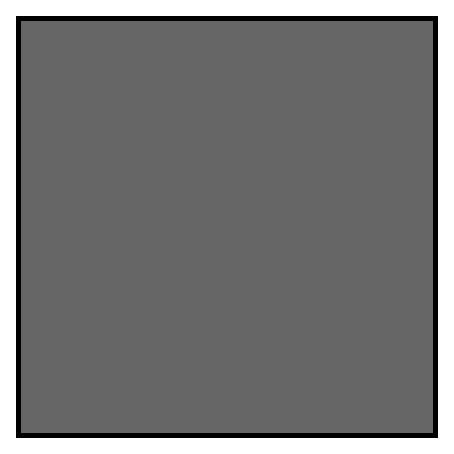
\includegraphics{example.eps}
% % figure caption is below the figure
% \caption{Please write your figure caption here}
% \label{fig:1}       % Give a unique label
% \end{figure}
% %
% % For two-column wide figures use
% \begin{figure*}
% % Use the relevant command to insert your figure file.
% % For example, with the graphicx package use
%   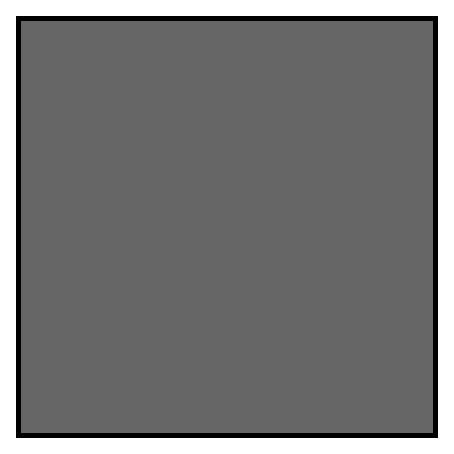
\includegraphics[width=0.75\textwidth]{example.eps}
% % figure caption is below the figure
% \caption{Please write your figure caption here}
% \label{fig:2}       % Give a unique label
% \end{figure*}
% %
% % For tables use
% \begin{table}
% % table caption is above the table
% \caption{Please write your table caption here}
% \label{tab:1}       % Give a unique label
% % For LaTeX tables use
% \begin{tabular}{lll}
% \hline\noalign{\smallskip}
% first & second & third  \\
% \noalign{\smallskip}\hline\noalign{\smallskip}
% number & number & number \\
% number & number & number \\
% \noalign{\smallskip}\hline
% \end{tabular}
% \end{table}


% %\begin{acknowledgements}
% %If you'd like to thank anyone, place your comments here
% %and remove the percent signs.
% %\end{acknowledgements}


% % Authors must disclose all relationships or interests that 
% % could have direct or potential influence or impart bias on 
% % the work: 
% %
% % \section*{Conflict of interest}
% %
% % The authors declare that they have no conflict of interest.


% % BibTeX users please use one of
% %\bibliographystyle{spbasic}      % basic style, author-year citations
% %\bibliographystyle{spmpsci}      % mathematics and physical sciences
% %\bibliographystyle{spphys}       % APS-like style for physics
% %\bibliography{}   % name your BibTeX data base

% % Non-BibTeX users please use
% \begin{thebibliography}{}
% %
% % and use \bibitem to create references. Consult the Instructions
% % for authors for reference list style.
% %
% \bibitem{RefJ}
% % Format for Journal Reference
% Author, Article title, Journal, Volume, page numbers (year)
% % Format for books
% \bibitem{RefB}
% Author, Book title, page numbers. Publisher, place (year)
% % etc
% \end{thebibliography}

\end{document}
% end of file template.tex

